\documentclass[11pt]{beamer}
%\useoutertheme{infolines}
\usetheme{Montpellier}
\usepackage[utf8]{inputenc}
\usepackage{amsmath}
\usepackage{amsfonts}
\usepackage{amssymb}
\usepackage{graphicx}
\usepackage{array}

%\setbeamercovered{transparent} 
\setbeamertemplate{navigation symbols}{} 
\logo{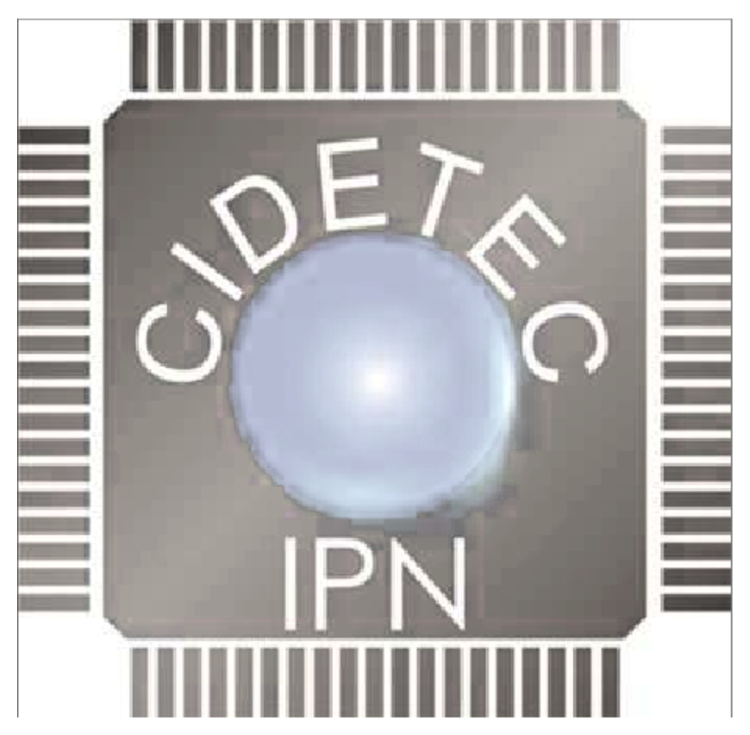
\includegraphics[width=.5cm]{Logos/logo_cidetec1.eps}
 \normalsize\insertframenumber} 

\title[Tesis]{\small\textbf{Sistema de aprendizaje no supervisado para la 
 detecci\'on y automatizaci\'on de tareas repetitivas en el entorno de una 
  computadora}}

\author[Gonz\'alez Tello]{
\textbf{\footnotesize Presenta:}\\
[0.1cm]{\footnotesize Ing.Ricardo Gonz\'alez Tello \\
[0.2cm] \footnotesize\textbf{Directores:} \\
[0.1cm] \footnotesize Dr. Jos\'e F\'elix S\'errano Talamantes \\
[0.1cm] \footnotesize Dr. Mauricio Olgu\'in Carbajal}
}

\date{\footnotesize México, Ciudad de México \hspace{2.5cm}
      \footnotesize Diciembre de 2018}


\begin{document}
\renewcommand{\tablename}{Tabla}
\renewcommand{\figurename}{Figura}

\begin{frame}
\begin{center}

    INSTITUTO POLIT\'{E}CNICO NACIONAL\\
	%\vspace{0.5cm}
    Centro de Innovaci\'on y Desarrollo
    Tecnol\'ogico en C\'omputo

\end{center}
\titlepage
\end{frame}

\begin{frame}
\frametitle{Contenido}
\footnotesize
\tableofcontents[hideothersubsections, subsubsectionstyle=hide]
\end{frame}

\section{Introducci\'on}

\begin{frame}
\frametitle{Introducci\'on}
\begin{figure}[h]
\centering
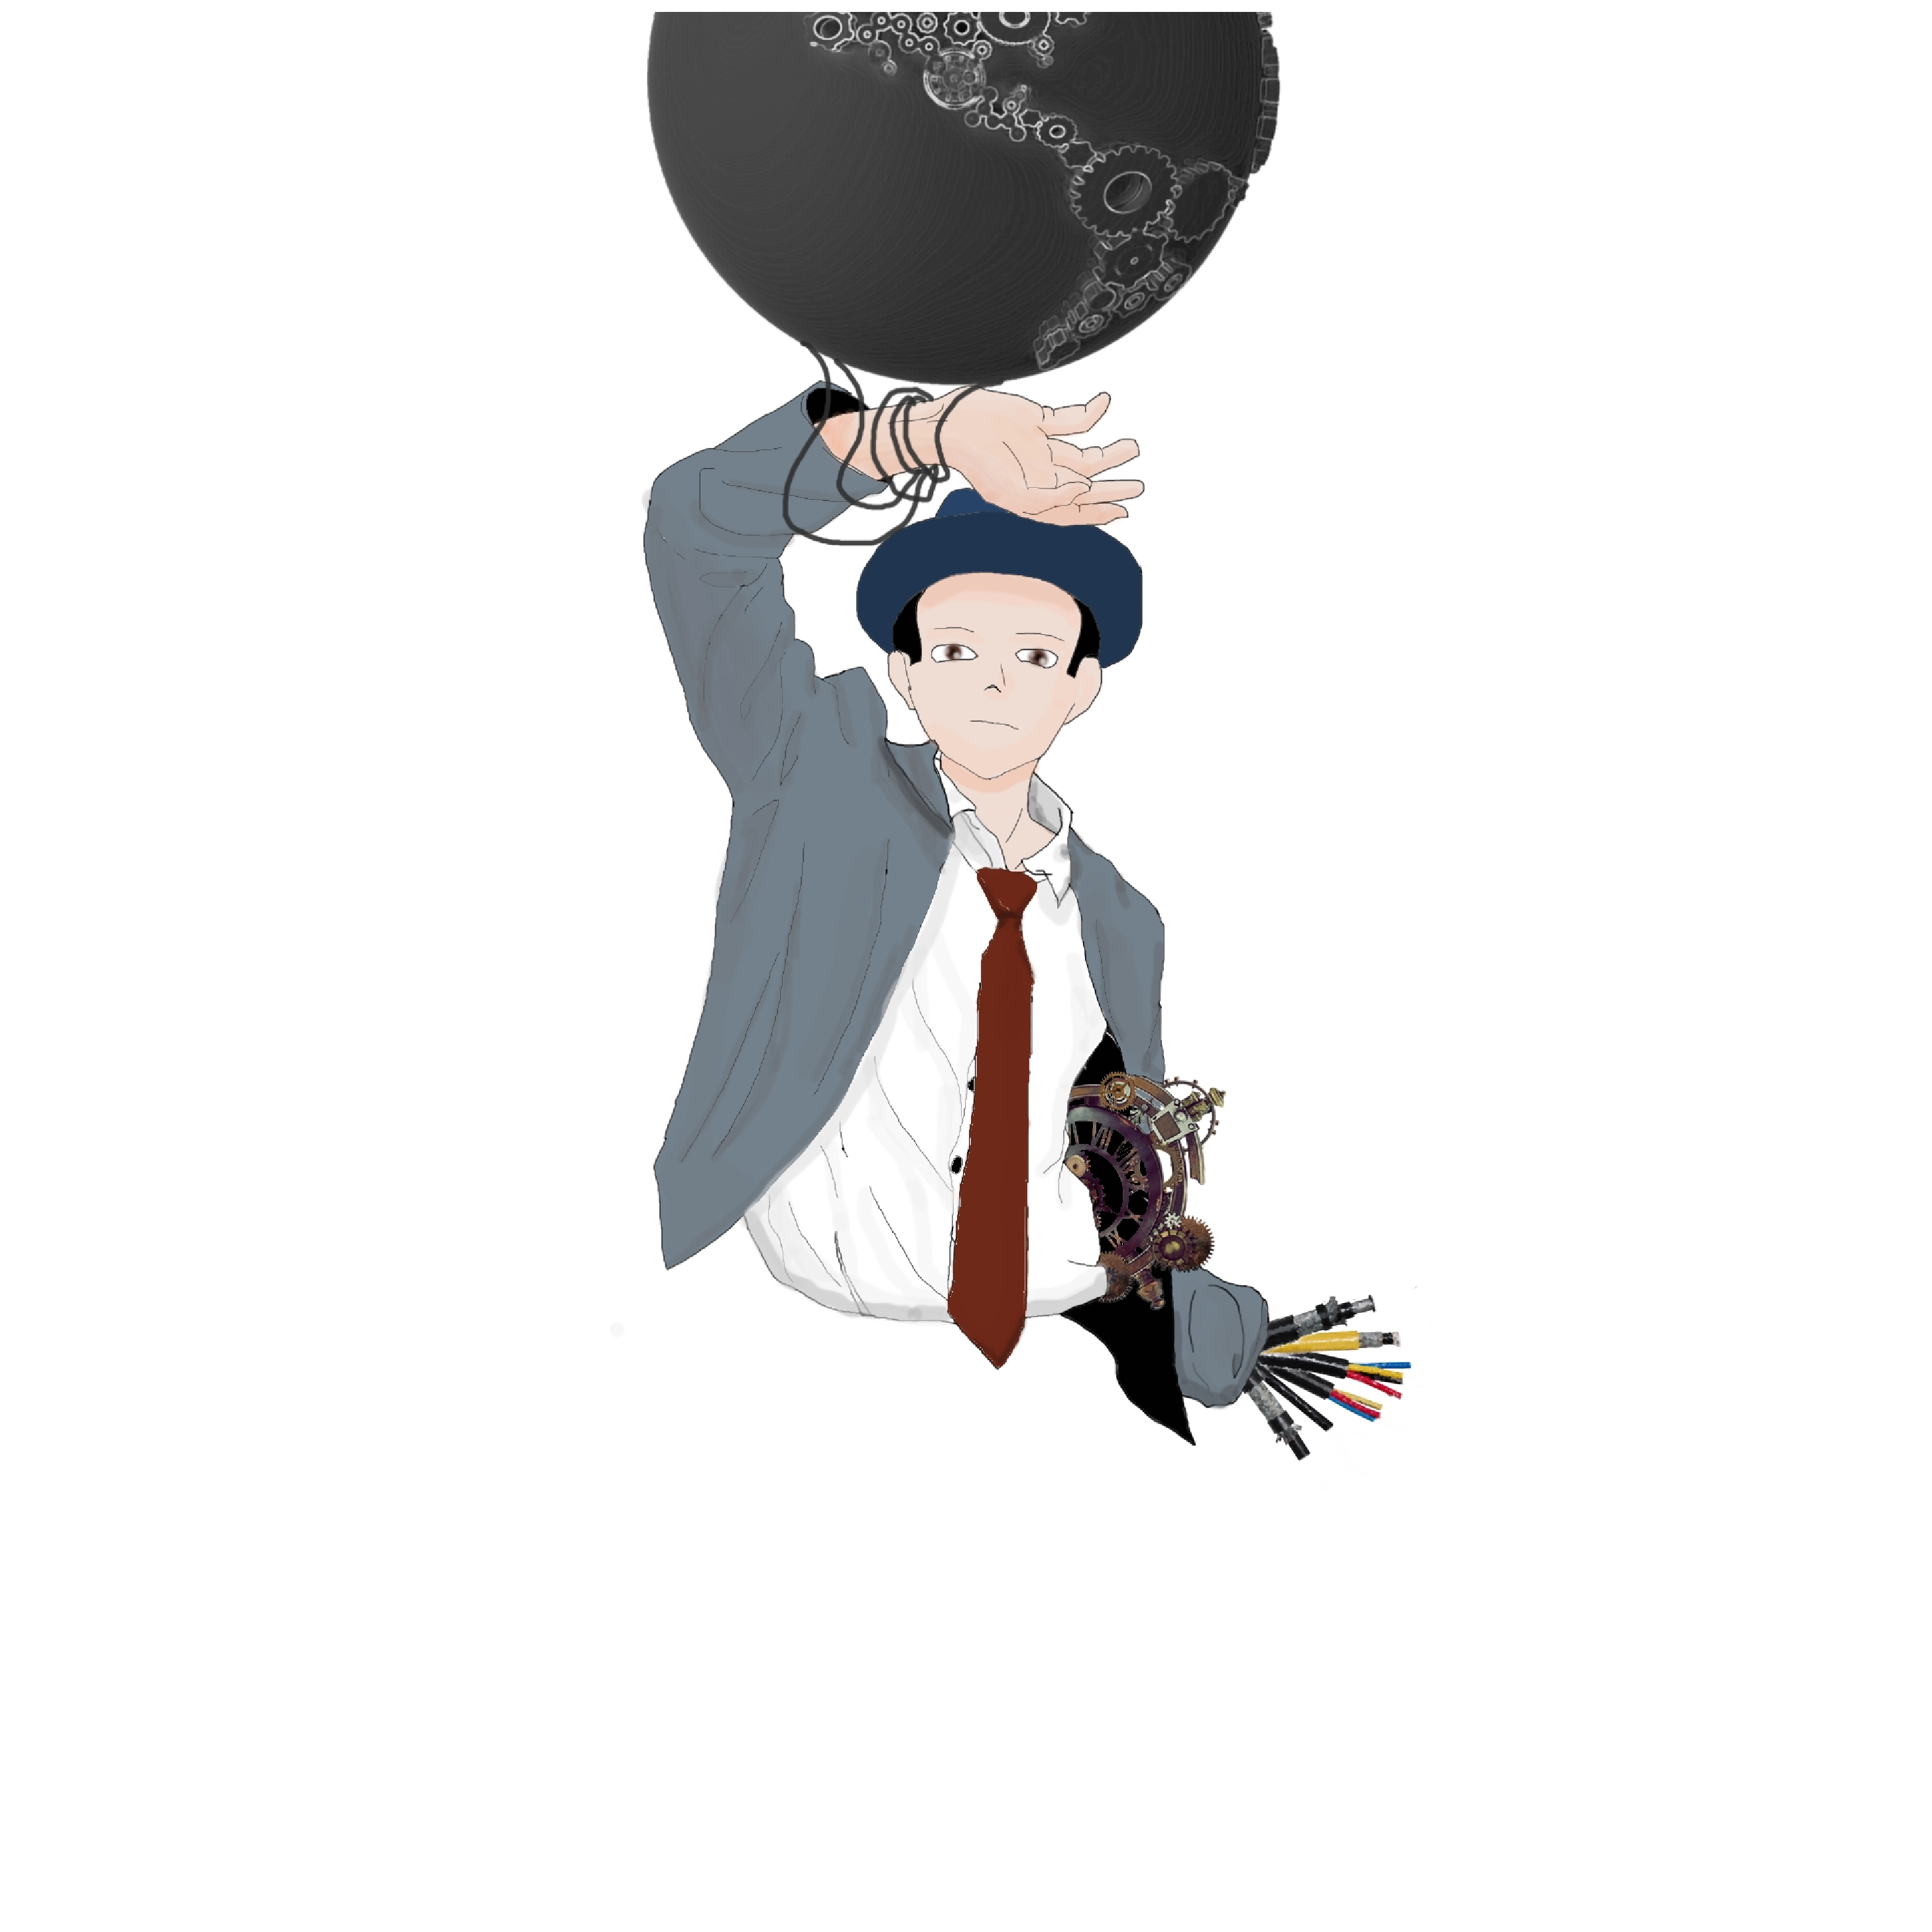
\includegraphics[width=0.85\columnwidth]{Imagenes/intro1.eps}
\end{figure} 
\end{frame}


\subsection{Justificaci\'on}
\begin{frame}
\frametitle{Justificaci\'on}

\begin{table}
\scalebox{0.75}{
\begin{tabular}{|l||c|c|c|}
\hline

\textbf{A\~no} & \textbf{2010} & \textbf{2012} & \textbf{2014} \\
\hline\hline

\textbf{Poblaci\'on Total} & $113.4$ M & $117.4$ M & $118.3$ M \\
\hline

\textbf{Poblaci\'on con Discapacidad} & $5.6$ M & $7.7$ M & $7.1$ M \\
\hline

\textbf{Porcentaje de Discapacidad} & $5.0\%$ & $6.6\%$ & $6.0\%$ \\
\hline

\end{tabular}
}
\caption{Poblaci\'on con discapacidad en M\'exico, seg\'un distintas fuentes
 \cite{Milosavljevic2014,INEGI2014}}
\label{PoblacionDis}
\end{table}


\begin{block}{Mover o usar sus brazos o manos -- $33.0\%$}
\begin{columns}[T]%{Mover o usar sus brazos o manos: $33.0\%$}
\begin{column}{.5\textwidth}
\begin{itemize}
\item {Enfermedad: $47.8\%$}
\item {Edad Avanzada: $29.2\%$}
\item {Accidente: $14.1\%$}
\end{itemize}
\end{column}
\begin{column}{.5\textwidth}
\begin{itemize}
\item {Nacimiento: $6.1\%$}
\item {Violencia: $0.5\%$}
\item {Otra causa: $2.3\%$}
\end{itemize}
\end{column}
\end{columns}
\end{block}

\end{frame}

\subsection{Planteamiento del problema}
\begin{frame}
\frametitle{Planteamiento del problema}

La poblaci\'on de Personas con Movilidad Reducida(PRM) va en aumento en 
 M\'exico  y con el uso de la computadora como algo imprescindible en la 
 actualidad, la discapacidad de estas personas puede representar un 
 obst\'aculo en su desarrollo laboral.

\end{frame}

\subsection{Hip\'otesis}
\begin{frame}
\frametitle{Hip\'otesis}

El ser humano es un ser de costumbres, por lo que hay tareas repetitivas
 que son automatizables, por tal, el uso del software a desarrollar
 permitir\'a al usuario de la PC agilizar este tipo de tareas, ayudando con 
 un manejo m\'as \'agil del equipo.

\end{frame}

\subsection{Propuesta de trabajo}
\begin{frame}
\frametitle{Propuesta de trabajo}

\footnotesize
\begin{itemize}
\item{Interacci\'on con todos los programas de un usuario}
\item{Facilidad de uso}
\item{Automatizar las acciones de un usuario}
\end{itemize}

\begin{figure}[h]
\centering
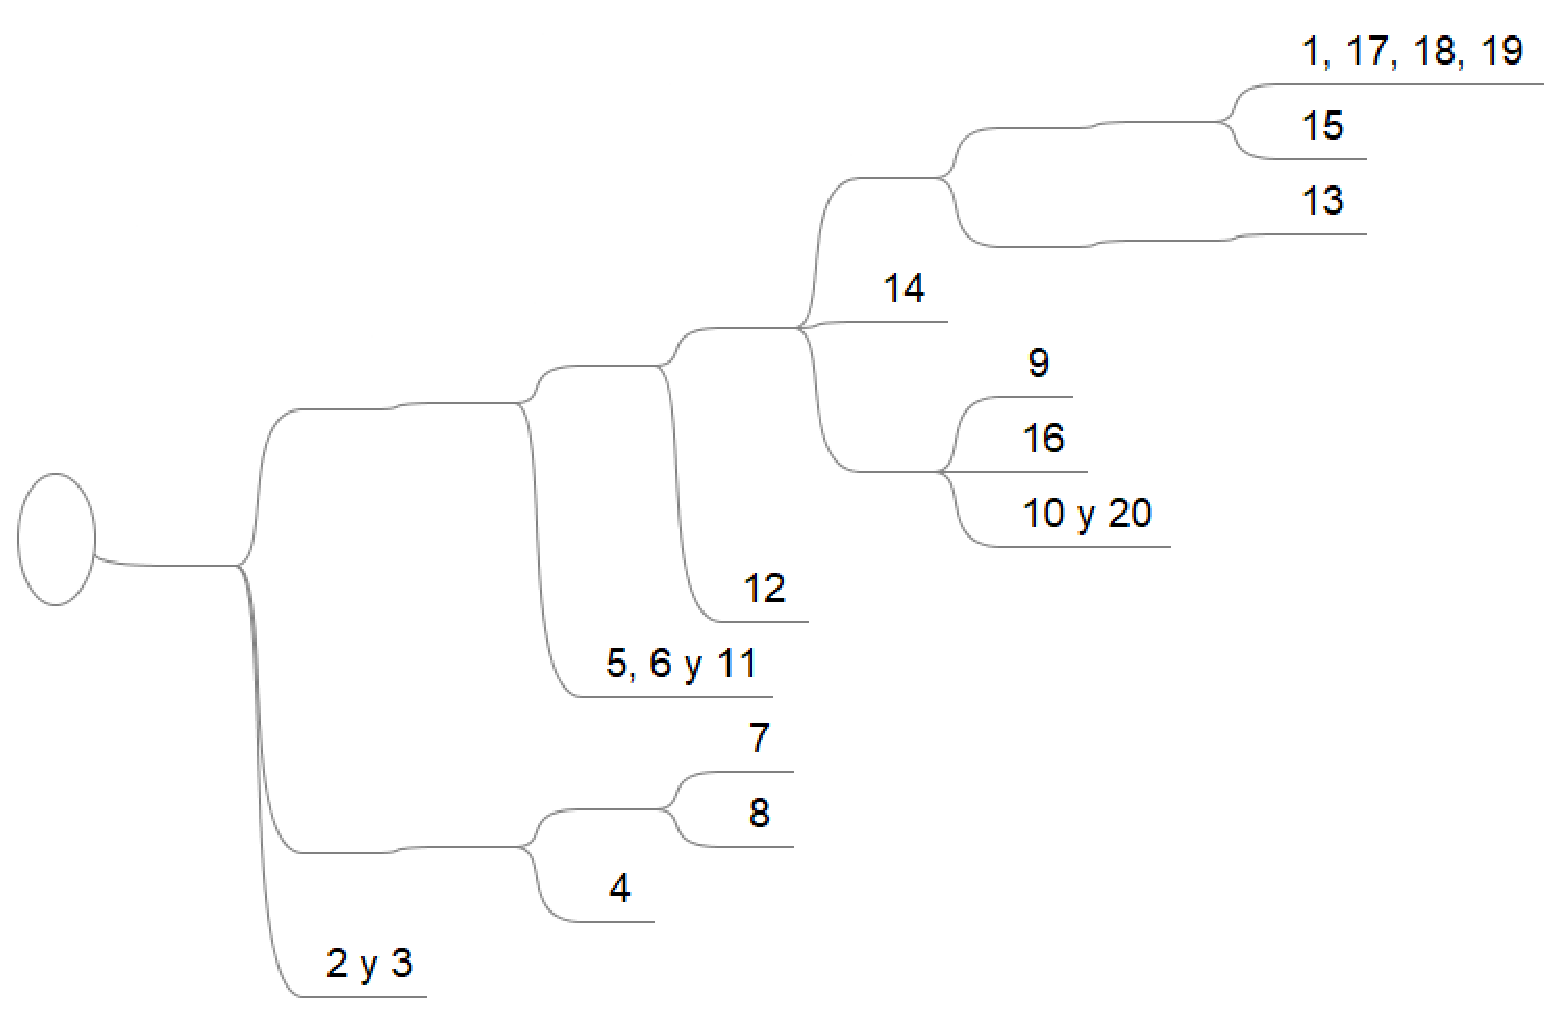
\includegraphics[width=0.6\columnwidth]{Imagenes/Arbol.eps}
\caption{\footnotesize Ejemplo del \'arbol ideal generado al pasar 20 d\'ias
 de uso en una PC.}
\label{fig:arbol}
\end{figure}

\end{frame}


\subsection{Objetivos} 
\begin{frame}
\frametitle{Objetivo general} 

Dise\~nar y desarrollar un software que defina a partir de un periodo de
 tiempo determinado el conjunto de acciones con mayor incidencia de uso por 
 un usuario realizadas en una computadora por un usuario, para su uso 
 posterior.

\begin{block}{Objetivos espec\'ificos} 			
\begin{itemize}
  \item Desarrollar un sistema para la captura de acciones, tanto del rat\'on
  como del teclado.
  \item Crear e implementar un \'arbol para resolver el problema.
  \item Obtener una muestra de las acciones realizadas con el teclado y el 
  rat\'on por un usuario en una computadora.
  \item Dise\~nar y desarrollar el algoritmo para la determinaci\'on de
  tareas repetitivas.
\end{itemize}
\end{block}
	
\end{frame}

\section{Trabajos relacionados}

\begin{frame}
\frametitle{Antecedentes}
\begin{block}{Opciones de accesibilidad de Microsoft Windows
 \cite{DanielHubbell2016}}
\begin{itemize}
	\item Lupa.
	\item Narrador.
	\item Teclado en pantalla.
	\item Contraste alto.
	\item Reconocimiento de voz.
\end{itemize}
\end{block}

\begin{block}{Silla de ruedas VAHM3 \cite{Grasse2010}}

\end{block}
\end{frame}

\begin{frame}
\frametitle{Trabajos relacionados}

\begin{table}[!h]
\centering
\scalebox{0.65}{
\begin{tabular}{|p{3.5cm} || p{3.5cm} | p{3.5cm} | p{2.25cm} | p{2cm}|}
\hline

\textbf{Nombre del autor o del proyecto (A\~no)}
& \textbf{interacci\'on con todos los programas del usuario}
& \textbf{Metodolog\'ia empleada}
& \textbf{Automatizar acciones}
& \textbf{M\'ultiples tareas objetivo}
\\ 
\hline
\hline


\textbf{Microsoft Cortana\cite{support17214}(2014)}
& Solo de Microsoft
& Patentado
& Si
& Si
\\ 
\hline

\textbf{Archivo por lotes\cite{Silberschatz1999}(1960)}
& Solo el Sistema Operativo
& Scripts
& Si
& Si
\\ 
\hline

\textbf{Pulover\textsc{\char13}s Macro Creator\cite{Batista}(2013)}
& Si
& Scripts
& Si
& Si
\\ 
\hline

\textbf{UIPath\cite{Dines2018}(2005)}
& Si
& Robotic Process Automation
& Si
& Si
\\
\hline

\textbf{\emph{Propuesta}}
& \textbf{\emph{Si}}
& \textbf{\emph{Grafo}}
& \textbf{\emph{Si}}
& \textbf{\emph{Si}}
\\ 
\hline

\end{tabular}
}
\caption{Tabla de requisitos y an\'alisis comparativo}
\label{ComparativaT}
\end{table}
\end{frame} 
\section{Marco te\'orico}

\subsection{Machine learning}
\begin{frame}
\frametitle{Aprendizaje m\'aquina(Machine learning)}

\begin{figure}[h]
\centering
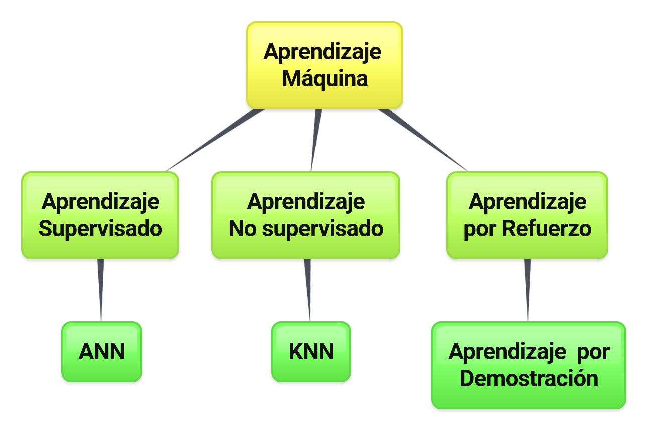
\includegraphics[width=0.8\columnwidth]{Imagenes/Aprendizaje.eps}
\caption{Clasificación del aprendizaje m\'aquina
 \cite{9780471056690, 9780387310732}.}
\label{fig:ClasifML}
\end{figure}

\end{frame} 


\subsection{Grafos}
\begin{frame}
\frametitle{Grafo dirigido}

\begin{figure}[h]
\centering
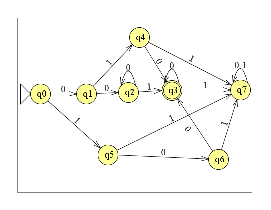
\includegraphics[width=0.7\columnwidth]{Imagenes/GrafoDirigido.eps}
\caption{Ejemplo de un grafo dirigido.}
\label{fig:grafod}
\end{figure}

\end{frame} 


\subsection{Tipos de datos}
\begin{frame}
\frametitle{Tipos de datos}

\begin{figure}[h]
\centering
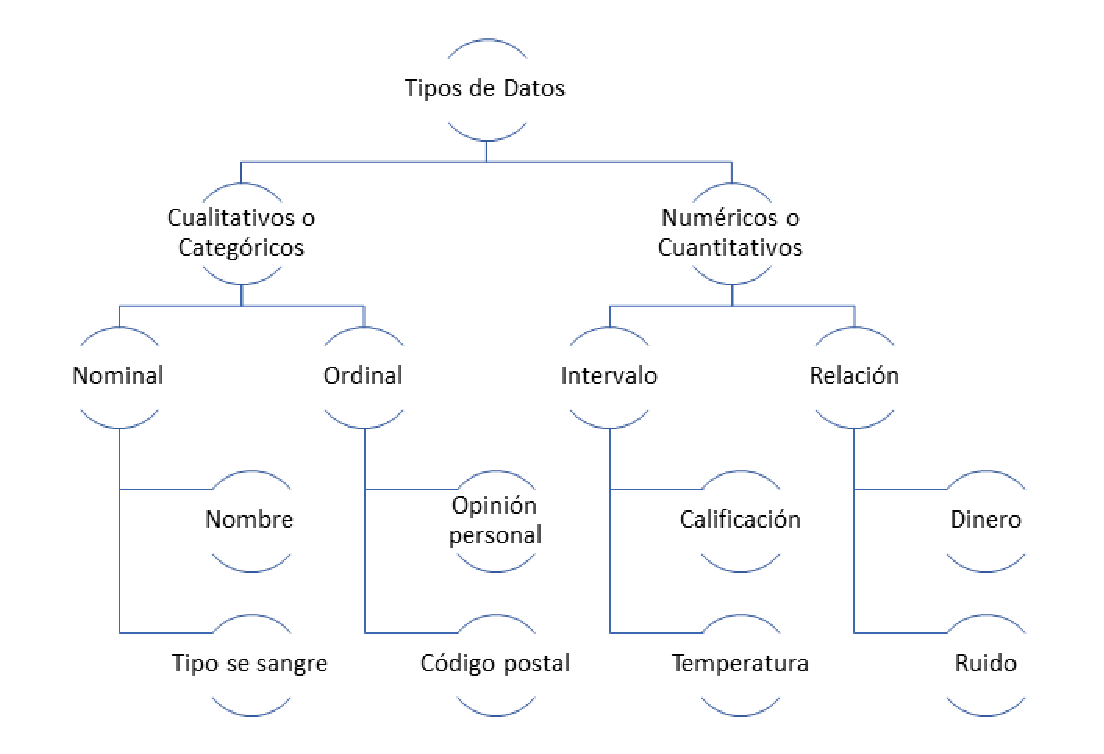
\includegraphics[width=0.85\columnwidth]{Imagenes/clasifnums.eps}
\caption{Clasificaci\'on de tipos de datos.}
\label{fig:clasnums}
\end{figure}

\end{frame}
\section{Desarrollo}

\subsection{Introducci\'on}
\begin{frame}
\frametitle{Introducci\'on}

\begin{figure}[h]
\centering
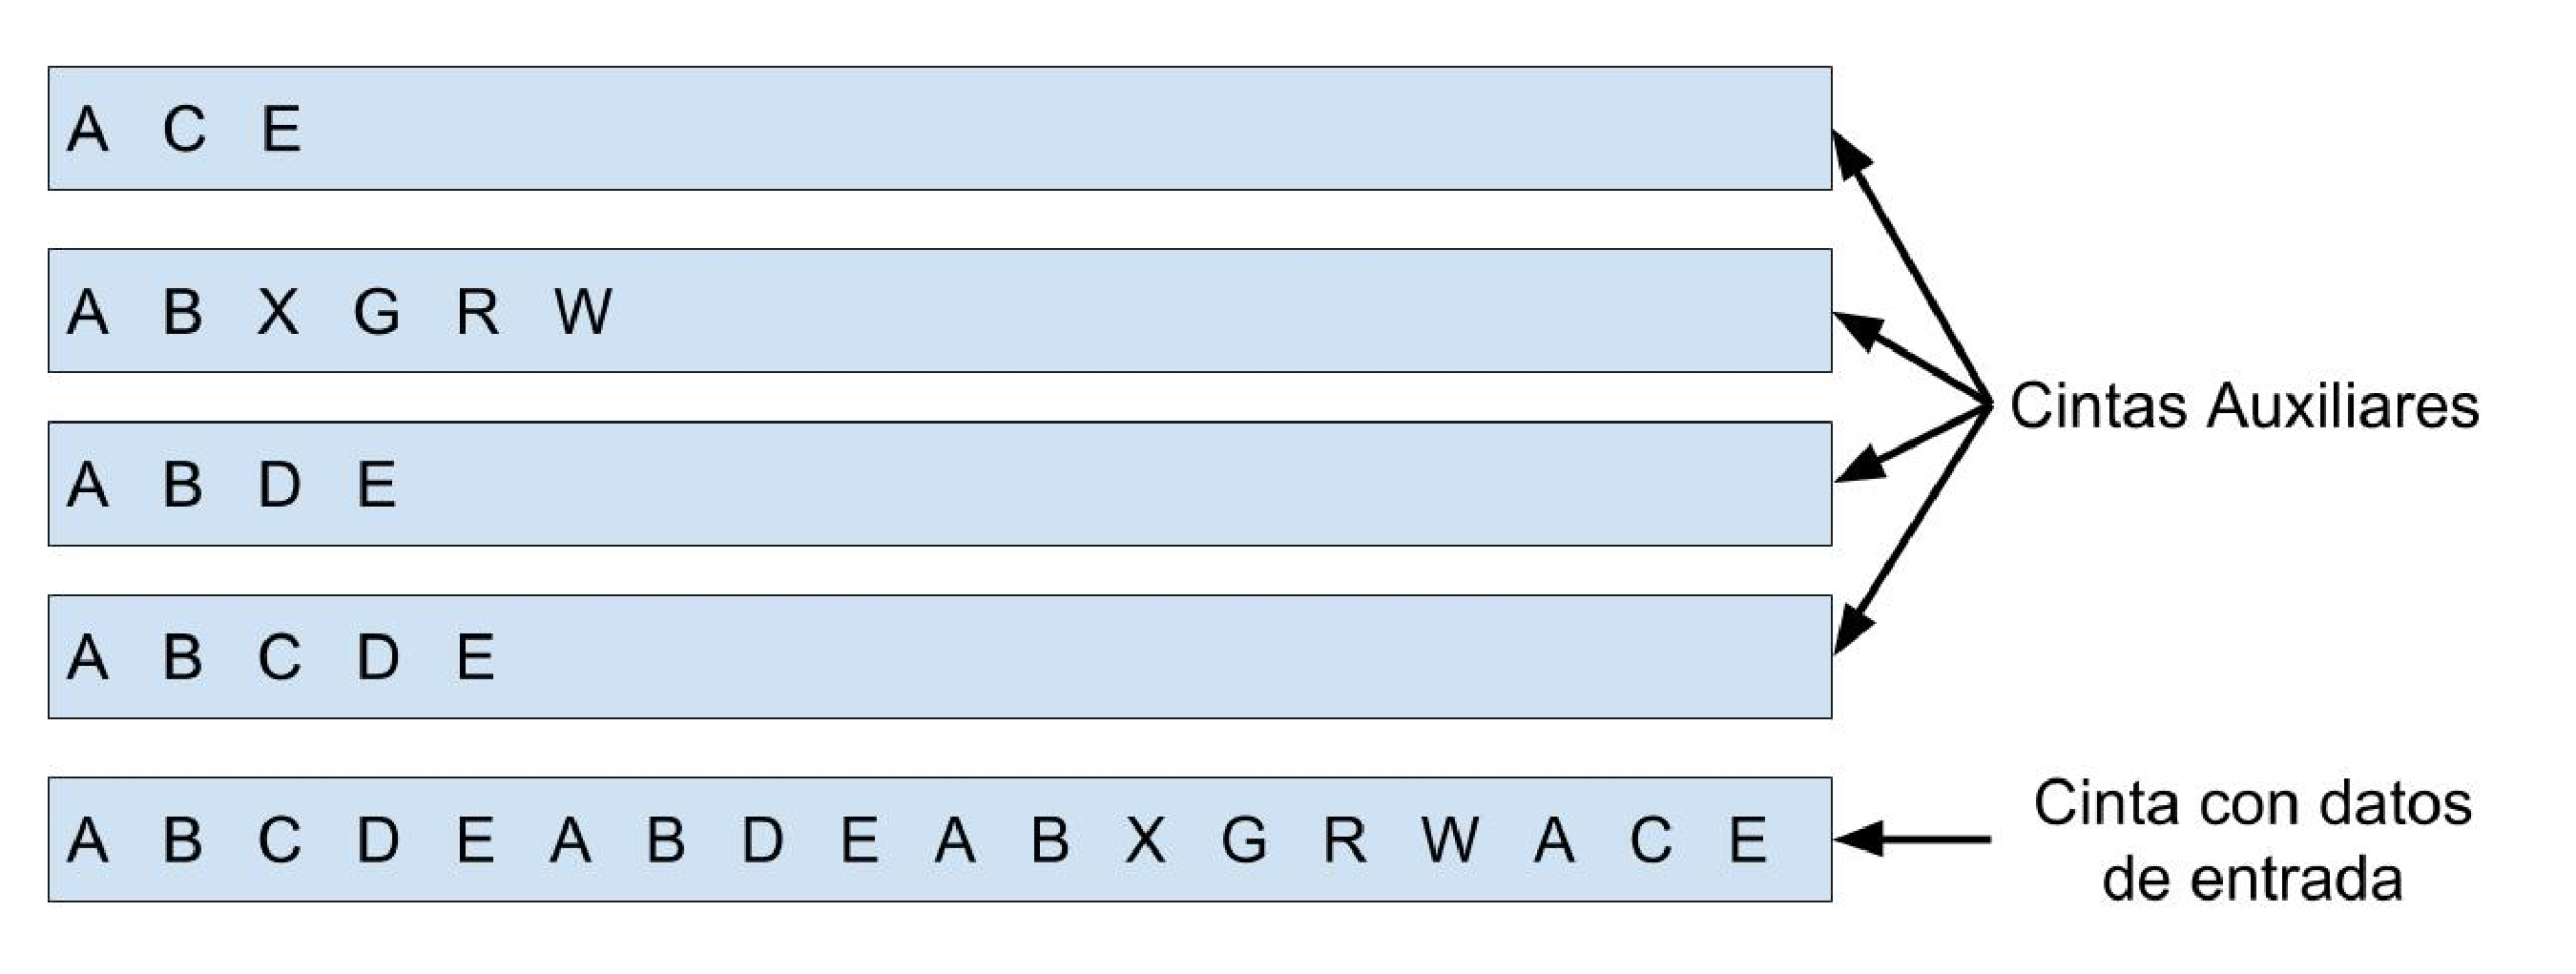
\includegraphics[width=1.0\columnwidth]{Imagenes/algoritmo1.eps}
\caption{Ejemplo del algoritmo con una m\'aquina de Turing multicinta.}
\label{fig:alg01}
\end{figure}

\end{frame}


\begin{frame}
\frametitle{Introducci\'on}

\begin{figure}[h]
\centering
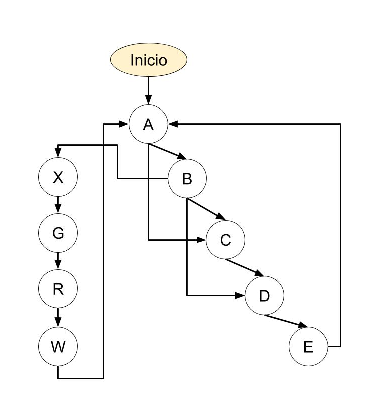
\includegraphics[width=0.5 \columnwidth]{Imagenes/algoritmo2.eps}
\caption{Ejemplo del algoritmo con un grafo dirigido.}
\label{fig:alg02}
\end{figure}

\end{frame}


\subsection{Desarrollo}
\begin{frame}
\frametitle{Vector de caracter\'isticas}

\begin{table}[!h]
\centering
\begin{tabular}{cccc}

\textbf{[Tiempo,} 
& \textbf{Dispositivo,} 
& \textbf{Acci\'on,}
& \textbf{Colocaci\'on]}
\\

& Keyboard
& Pressed
& Key
\\

& Mouse
& Release
& Button
\\

& 
& Scrolled
& Direction
\\

& 
& Moved
& Coordinates(X,Y)
\\


\end{tabular}
\end{table}

\begin{block}{\centering Muestra de acciones capturadas}
\centering
0.06,Mouse,Moved,1028,324\\
0.48,Mouse,Scrolled,Down\\
0.0,Keyboard,Pressed,Key.enter\\
\end{block}

\end{frame}


\begin{frame}
\frametitle{Funcionamiento}
\begin{figure}[H]
\centering
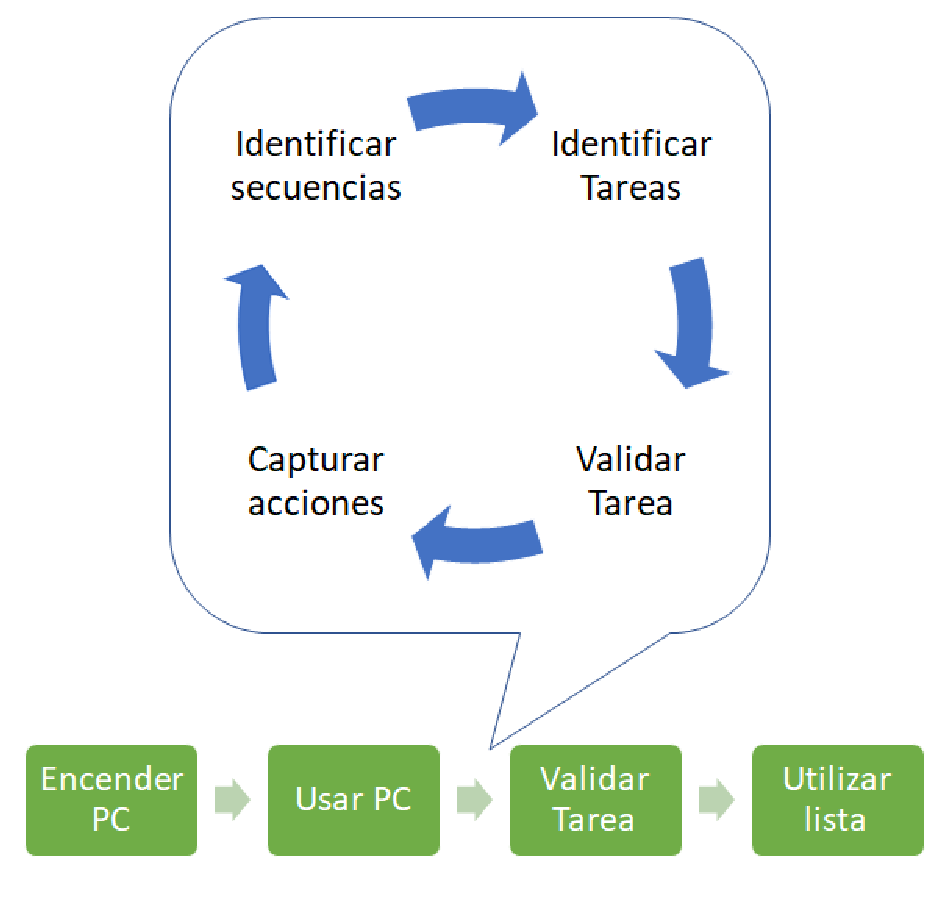
\includegraphics[width=0.6 \columnwidth]{Imagenes/Funcionamiento.eps}
\caption{Diagrama de funcionamiento.}
\label{fig:funcionamento}
\end{figure}
\end{frame}


\begin{frame}
\frametitle{Desarrollo}
\begin{figure}[h]
\centering
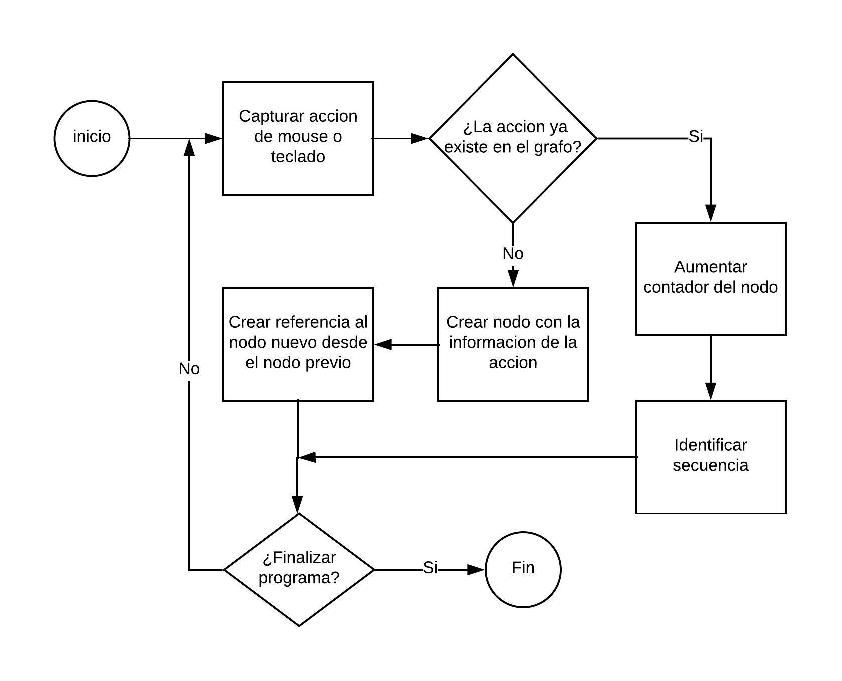
\includegraphics[height=0.55 \columnwidth]{Imagenes/Concepto1.eps}
\caption{Diagrama de flujo parte 1.}
\label{fig:bloques}
\end{figure}
\end{frame}

\begin{frame}
\frametitle{Desarrollo}
\begin{figure}[h]
\centering
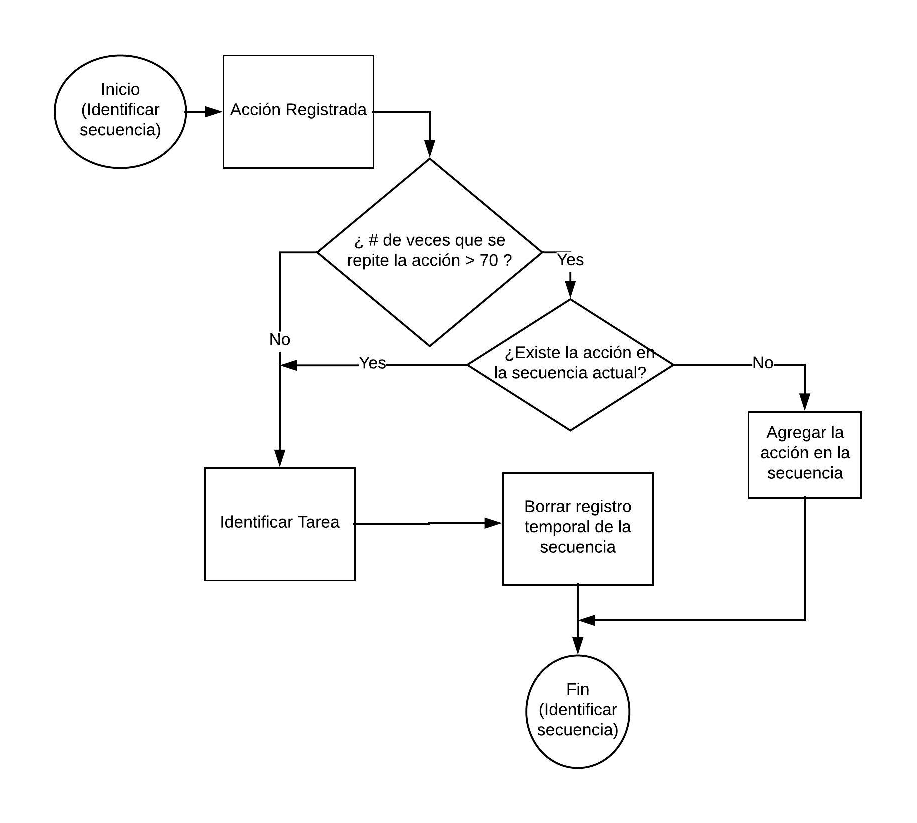
\includegraphics[height=0.55 \columnwidth]{Imagenes/Concepto2.eps}
\caption{Diagrama de flujo parte 2.}
\label{fig:bloques}
\end{figure}
\end{frame}

\begin{frame}
\frametitle{Desarrollo}
\begin{figure}[h]
\centering
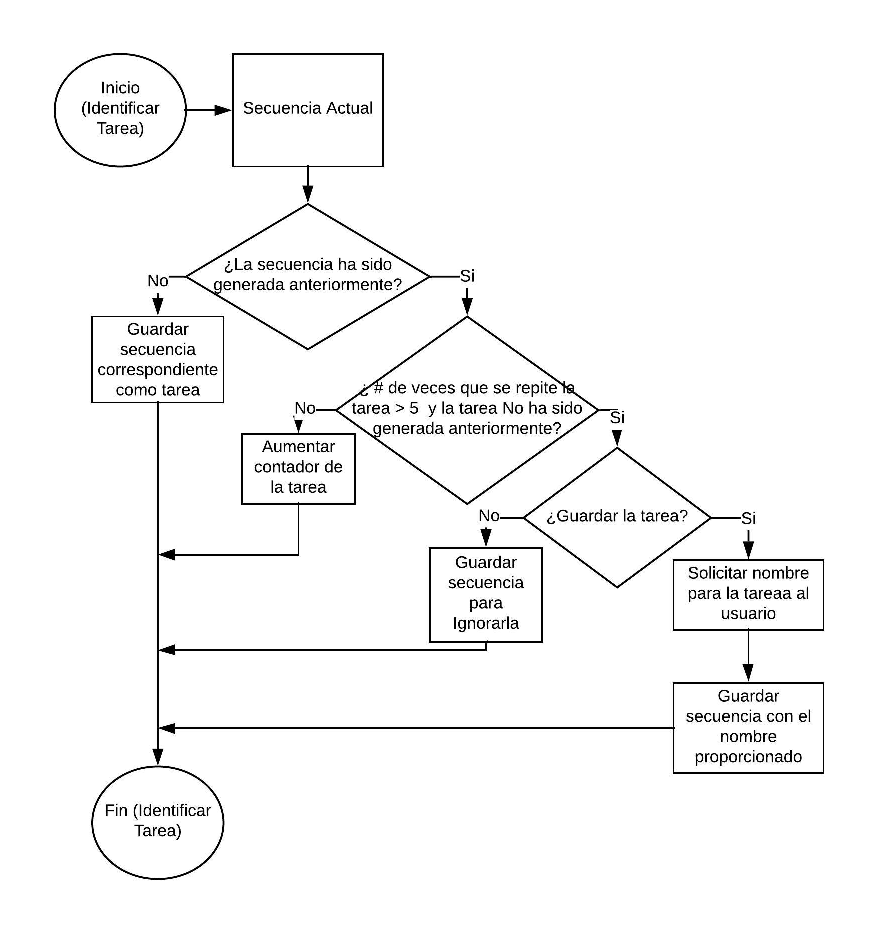
\includegraphics[height=0.55 \columnwidth]{Imagenes/Concepto3.eps}
\caption{Diagrama de flujo parte 3.}
\label{fig:bloques}
\end{figure}
\end{frame}


\begin{frame}
\frametitle{Interfaz Grafica}

\begin{figure}[H]
\centering
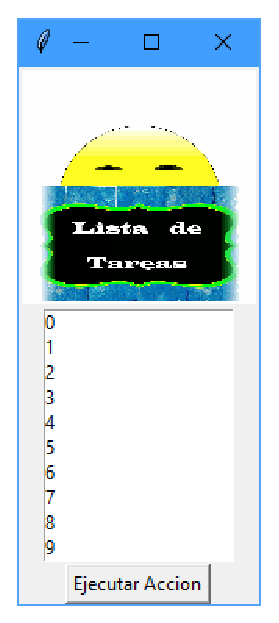
\includegraphics[width=0.2\columnwidth]{Imagenes/ventana1.eps}
\caption{Ventana principal con el asistente y una lista de tareas
 guardadas.}
\label{fig:v01}
\end{figure} 

\end{frame}


\begin{frame}
\frametitle{Interfaz Grafica}

\begin{figure}[H]
\centering
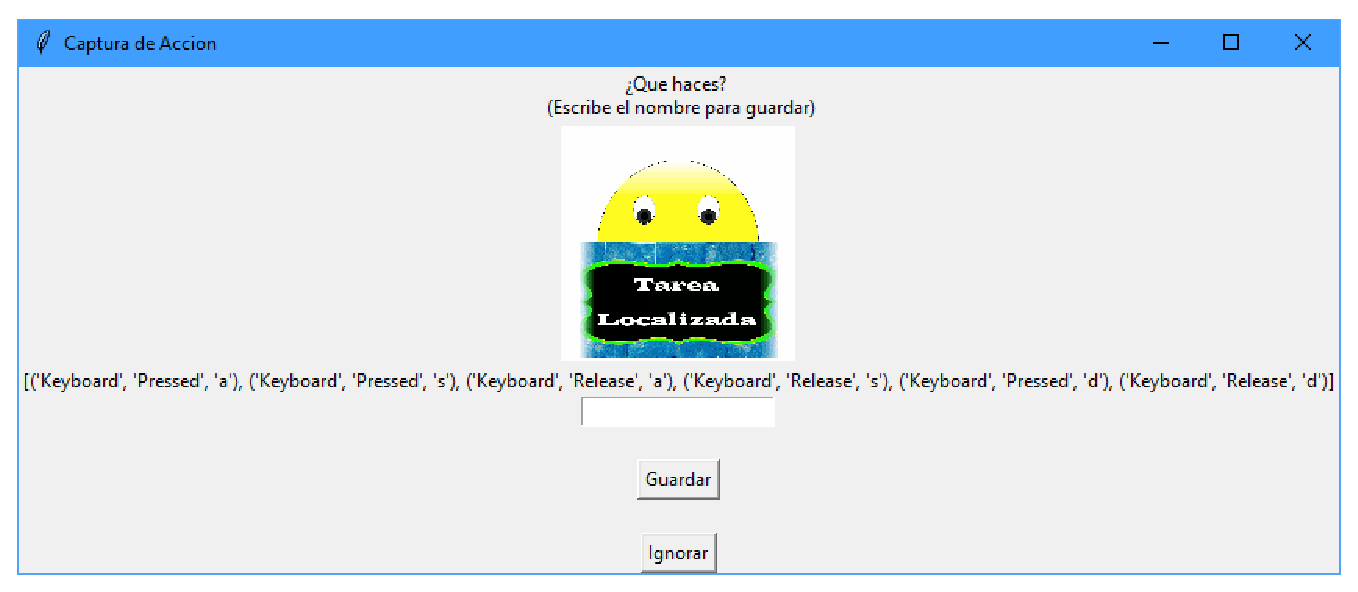
\includegraphics[width=1.0\columnwidth]{Imagenes/ventana2.eps}
\caption{Ventana mostrando una tarea encontrada.}
\label{fig:v02}
\end{figure}

\end{frame}

%-------------------------------------------------
\subsection{Demostraci\'on}

\begin{frame}
\frametitle{Demostraci\'on}
\begin{figure}[H]
\centering
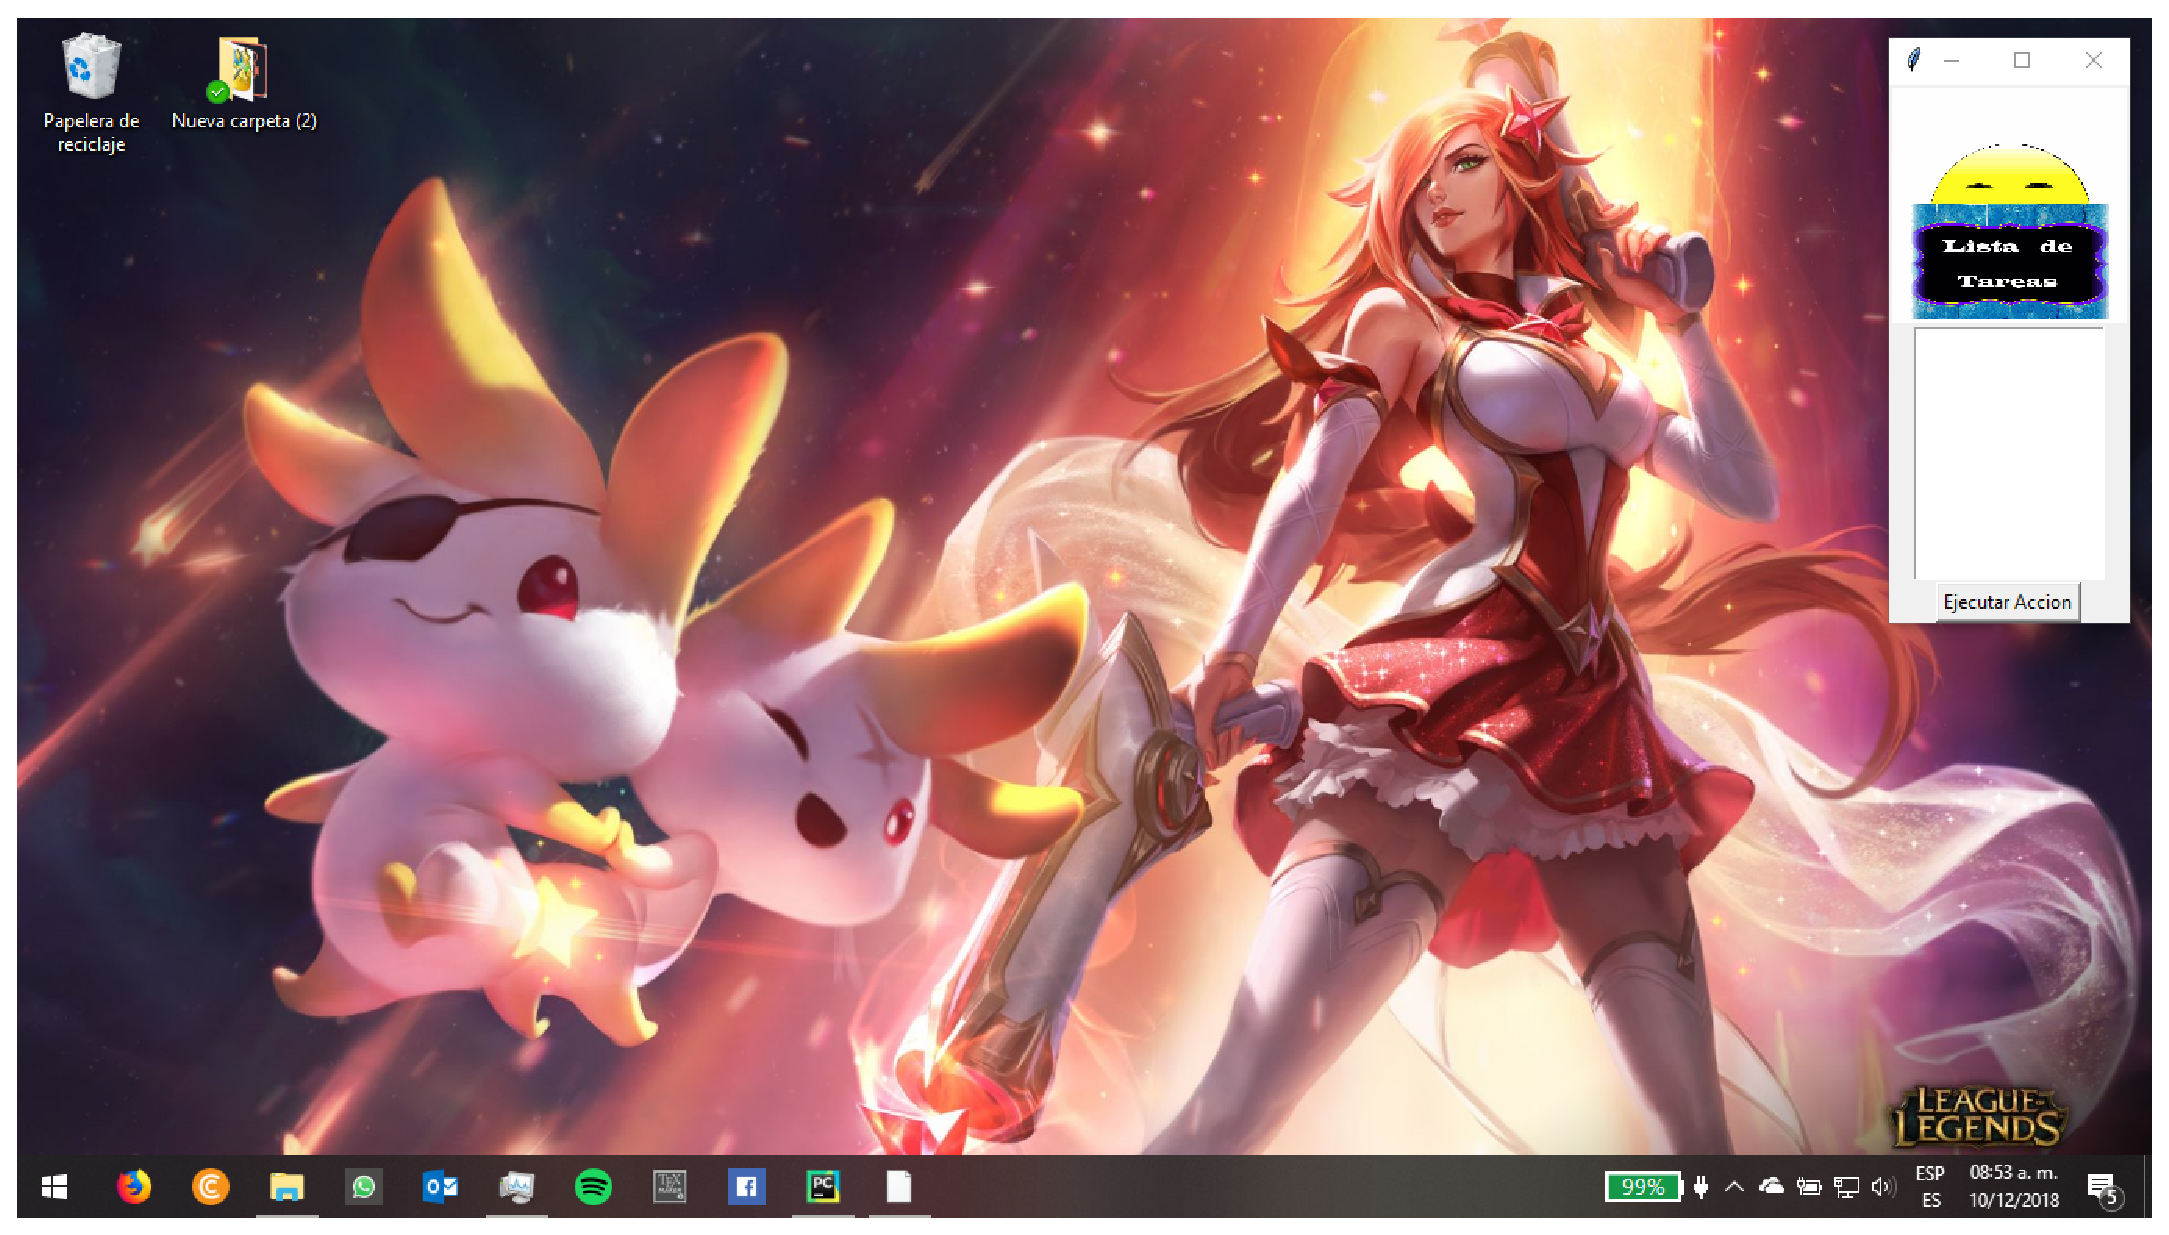
\includegraphics[width=1.0\columnwidth]{Imagenes/0.eps}
\end{figure}
\end{frame}

\begin{frame}
\frametitle{Demostraci\'on}
\begin{figure}[H]
\centering
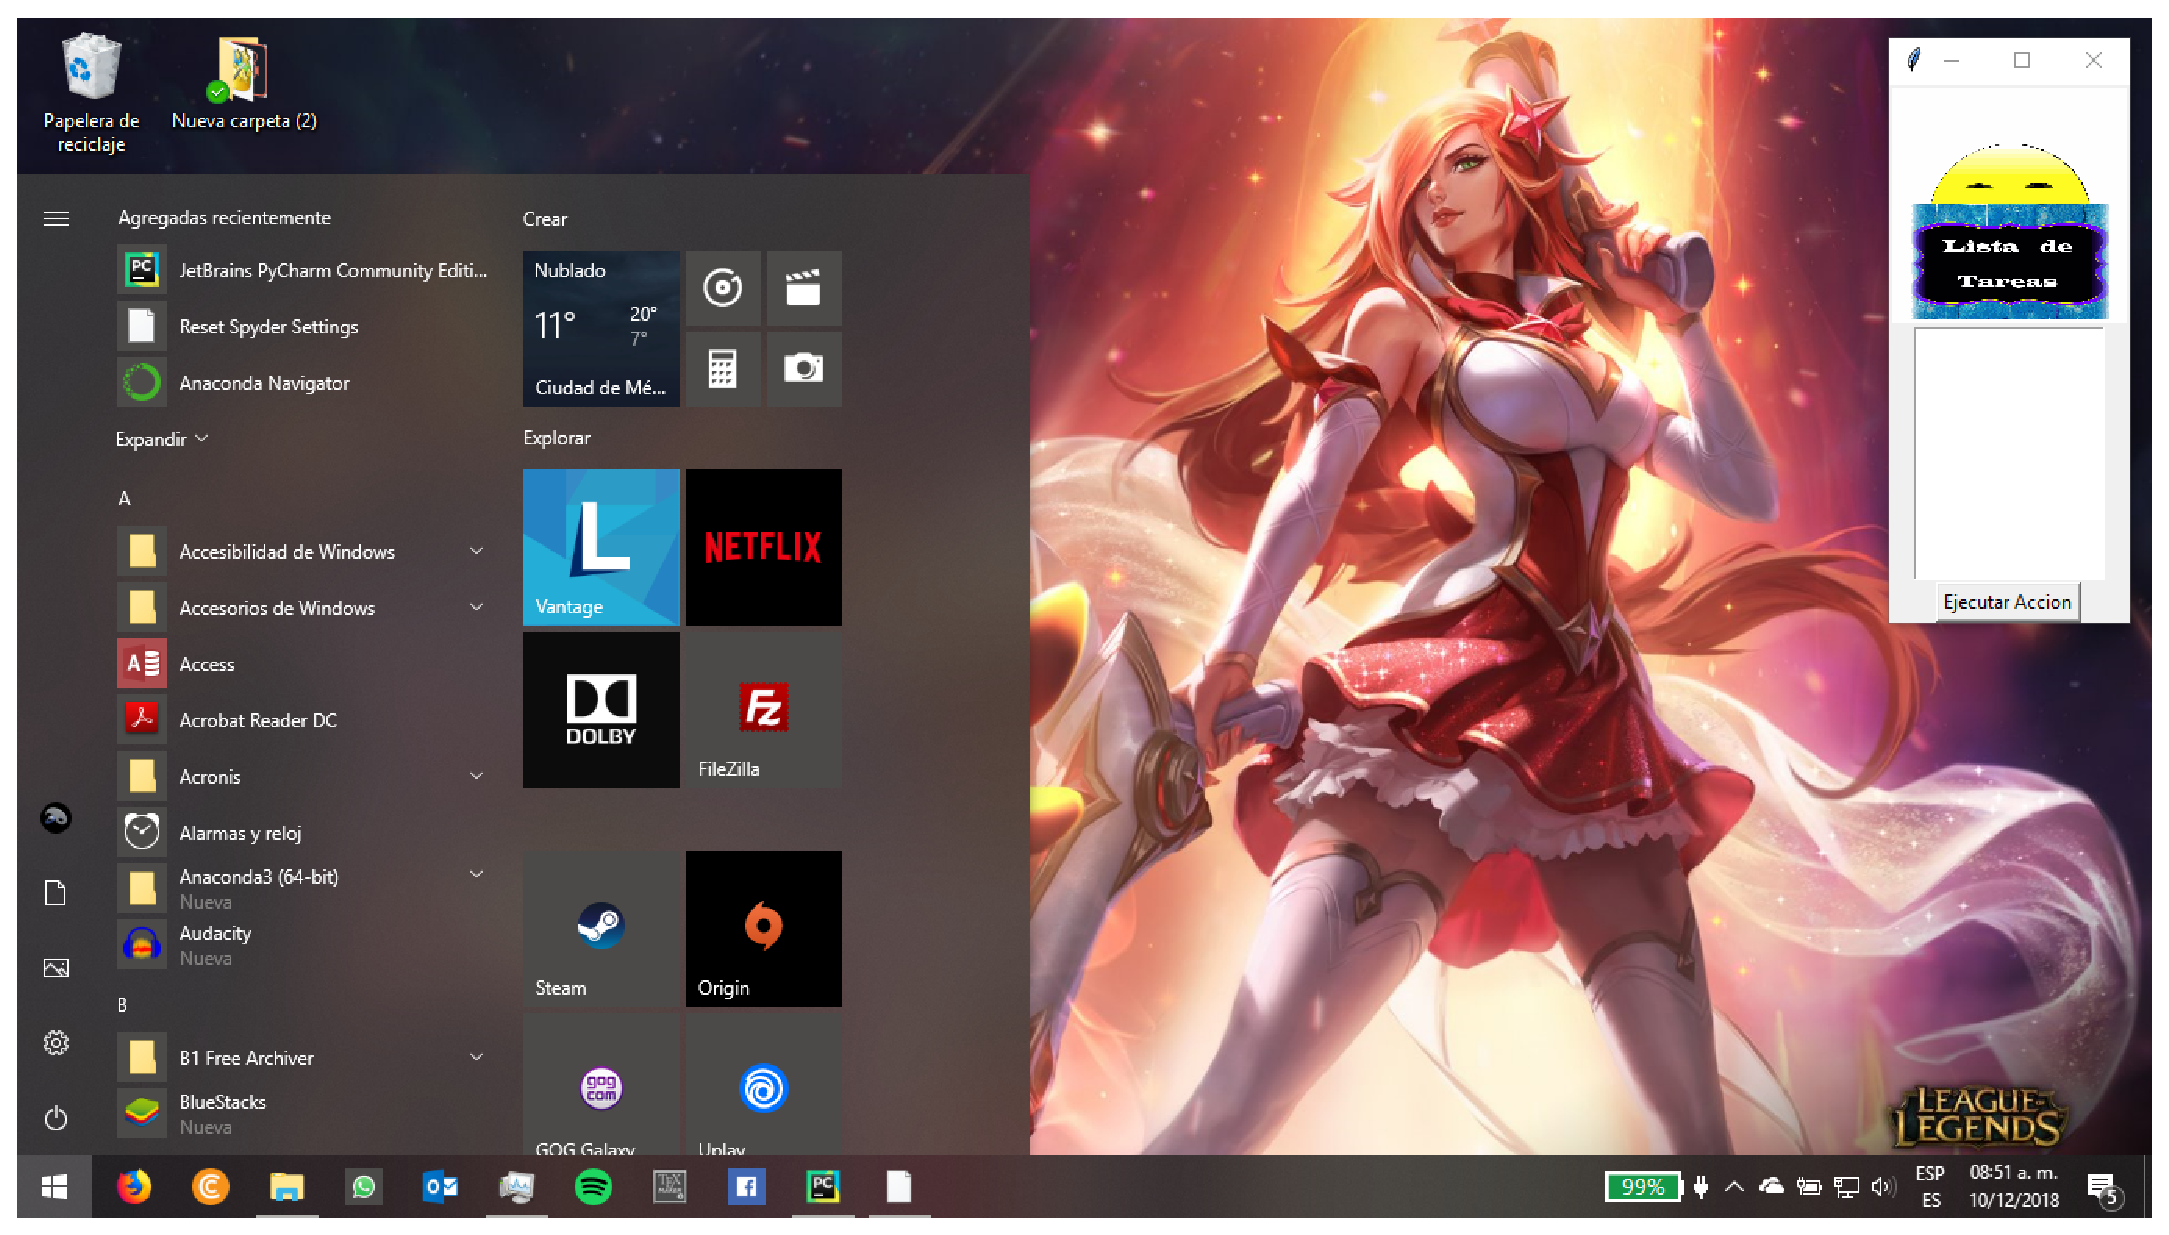
\includegraphics[width=1.0\columnwidth]{Imagenes/1.eps}
\end{figure}
\end{frame}

\begin{frame}
\frametitle{Demostraci\'on}
\begin{figure}[H]
\centering
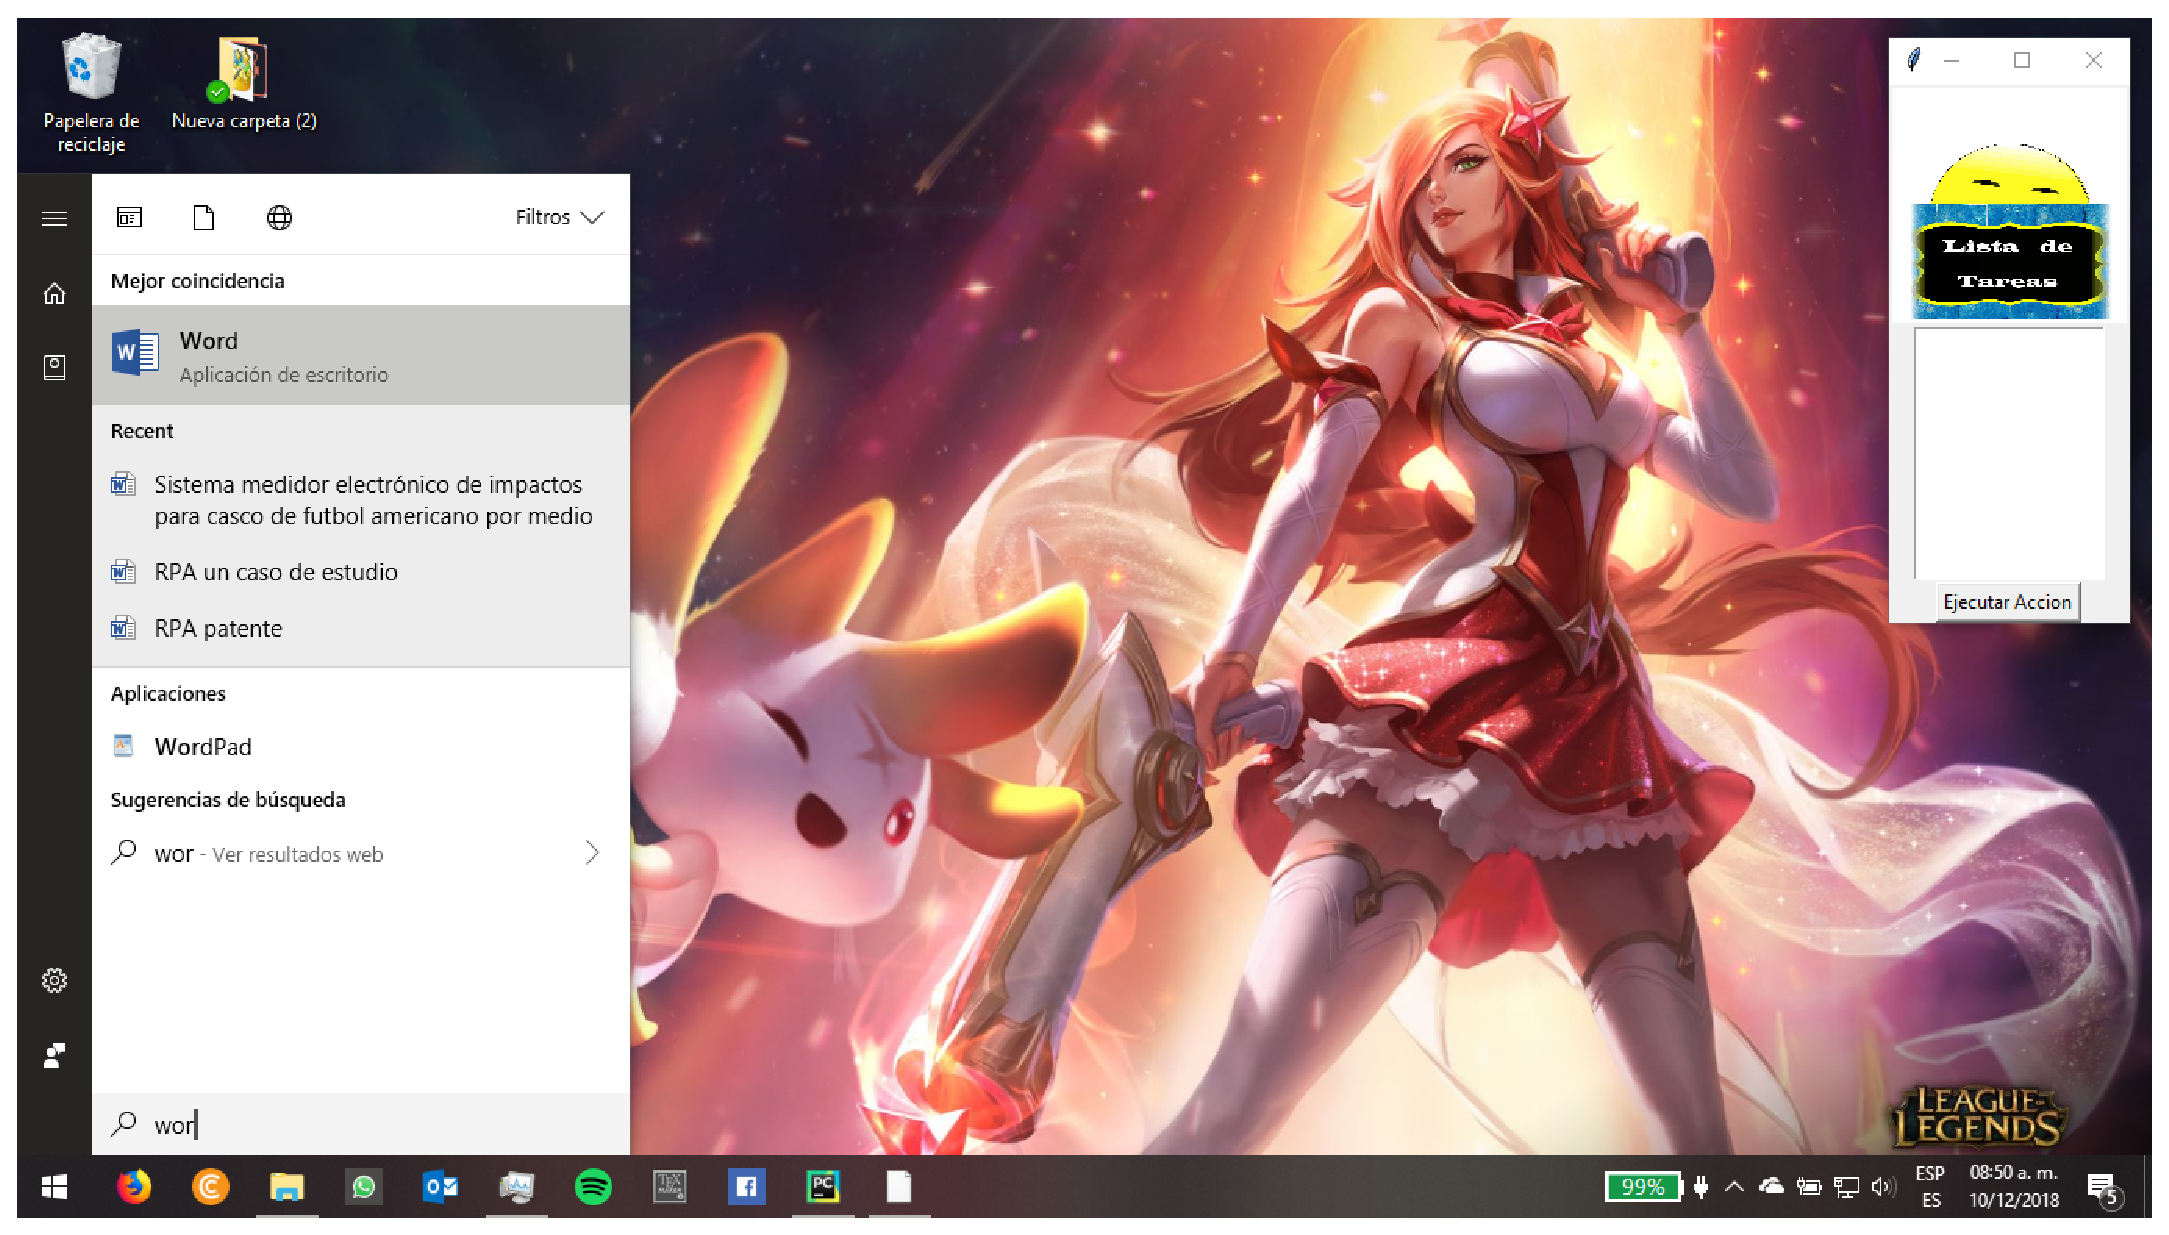
\includegraphics[width=1.0\columnwidth]{Imagenes/2.eps}
\end{figure}
\end{frame}

\begin{frame}
\frametitle{Demostraci\'on}
\begin{figure}[H]
\centering
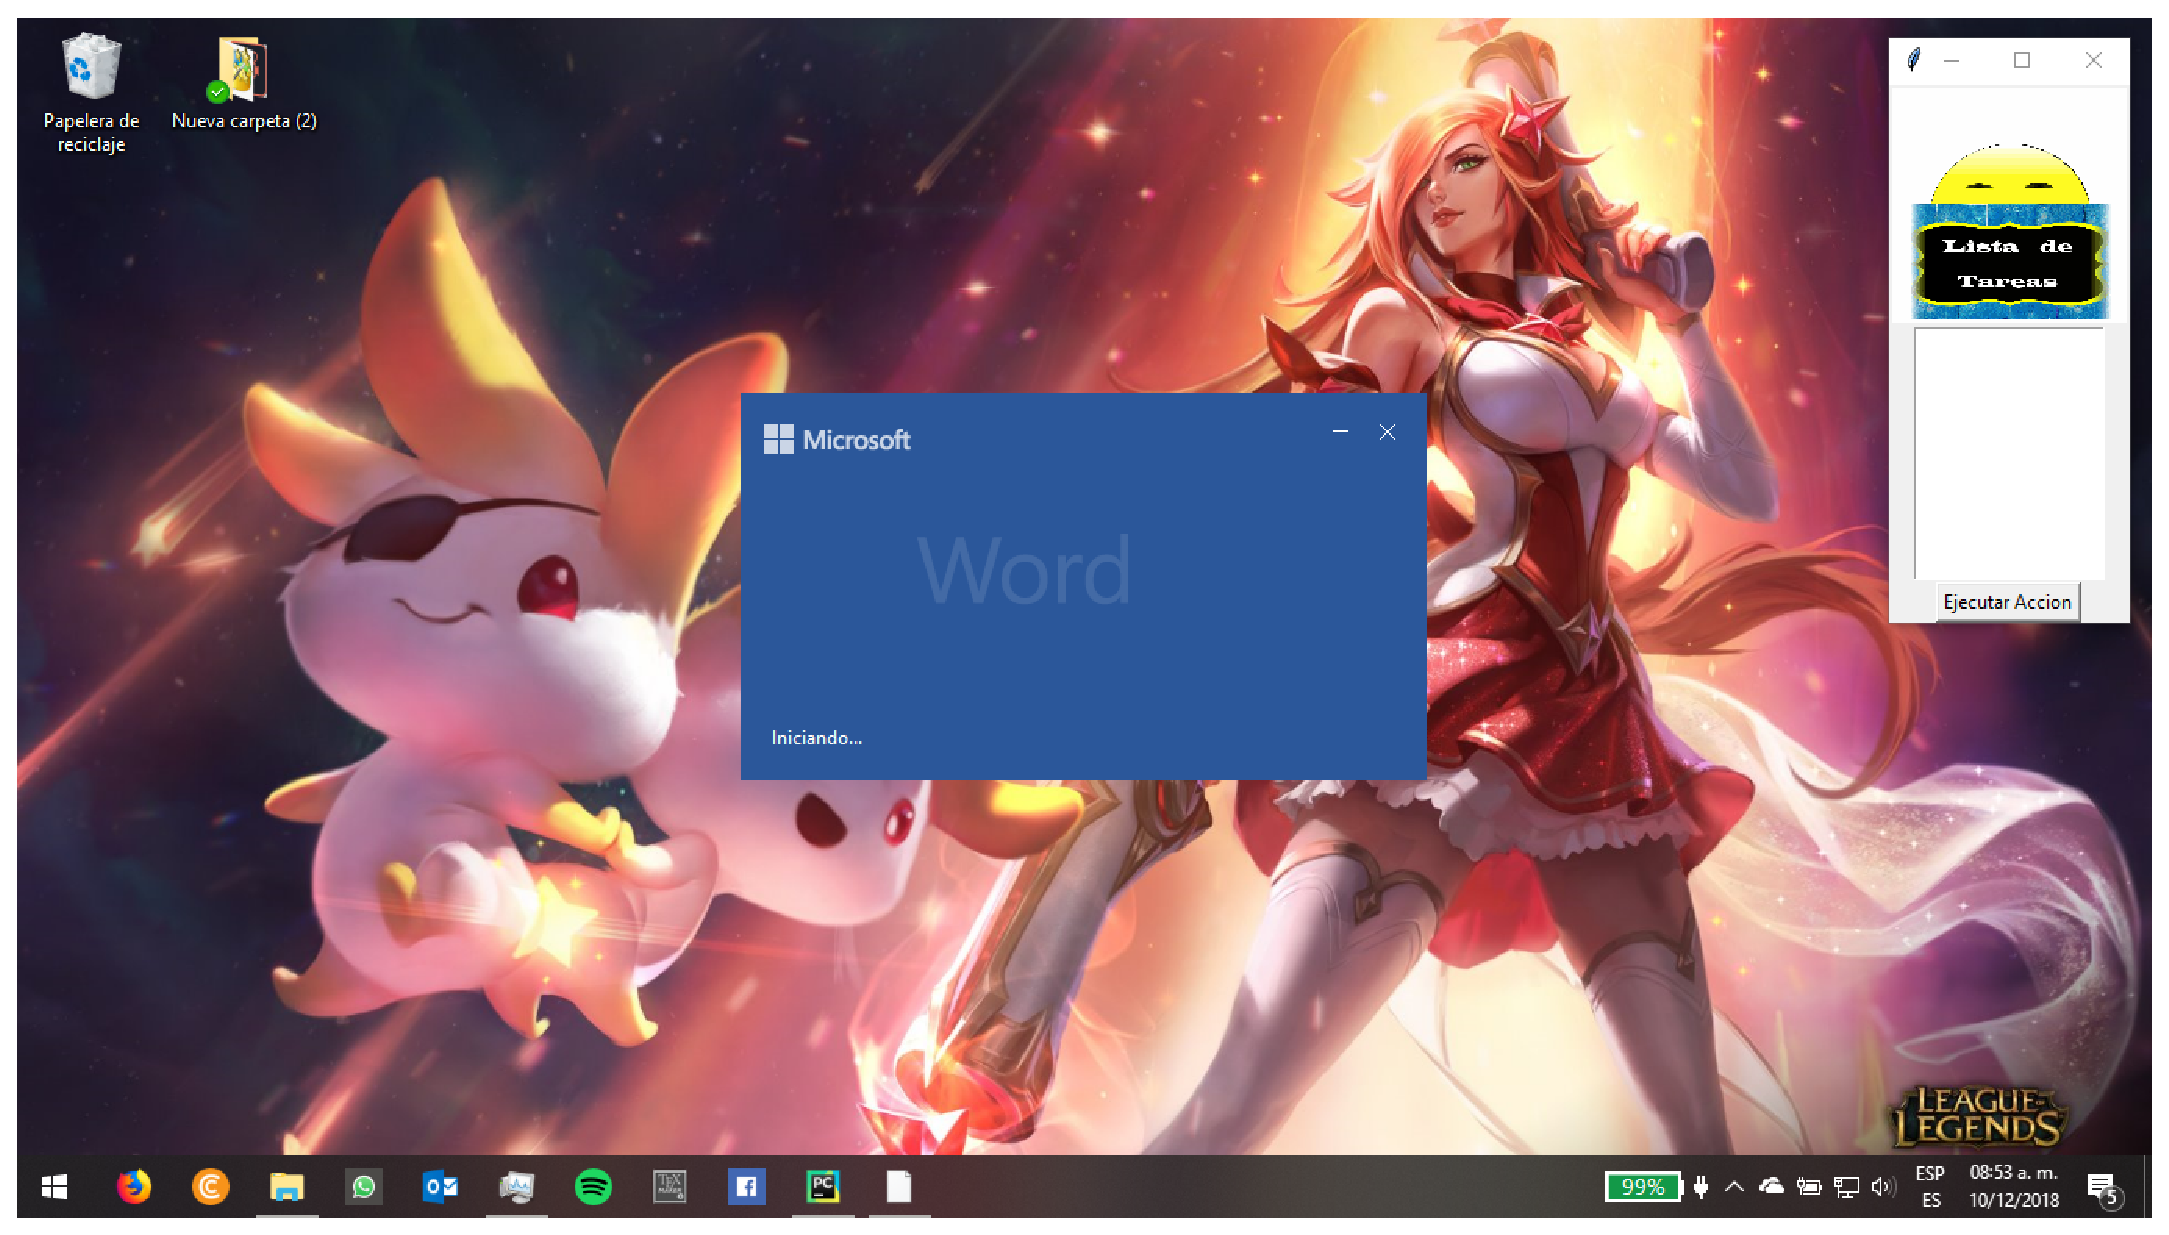
\includegraphics[width=1.0\columnwidth]{Imagenes/3.eps}
\end{figure}
\end{frame}

\begin{frame}
\frametitle{Demostraci\'on}
\begin{figure}[H]
\centering
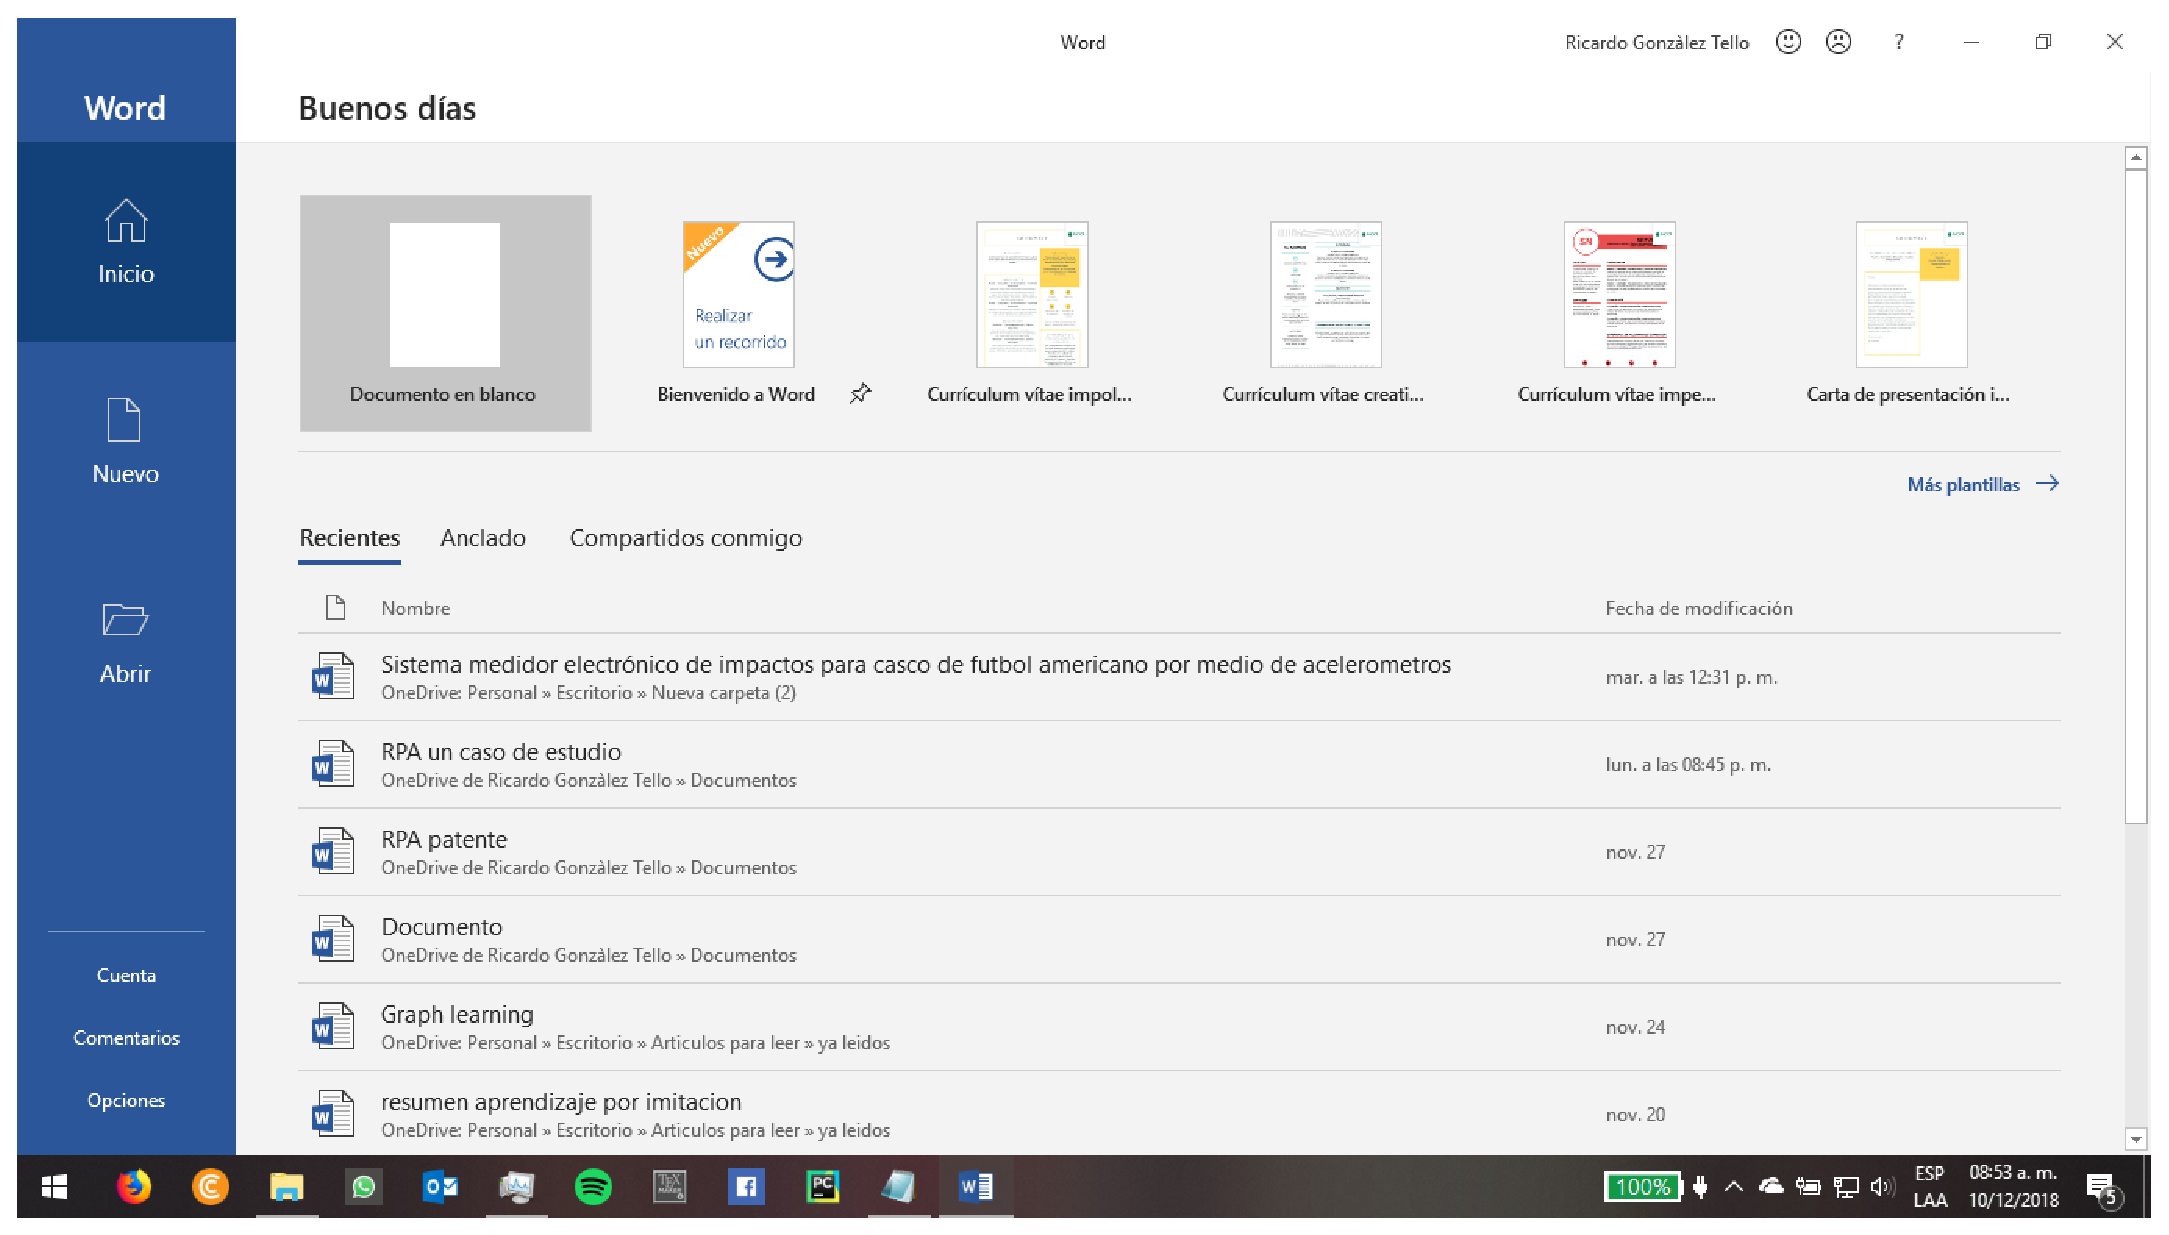
\includegraphics[width=1.0\columnwidth]{Imagenes/4.eps}
\end{figure}
\end{frame}

\begin{frame}
\frametitle{Demostraci\'on}
\begin{figure}[H]
\centering
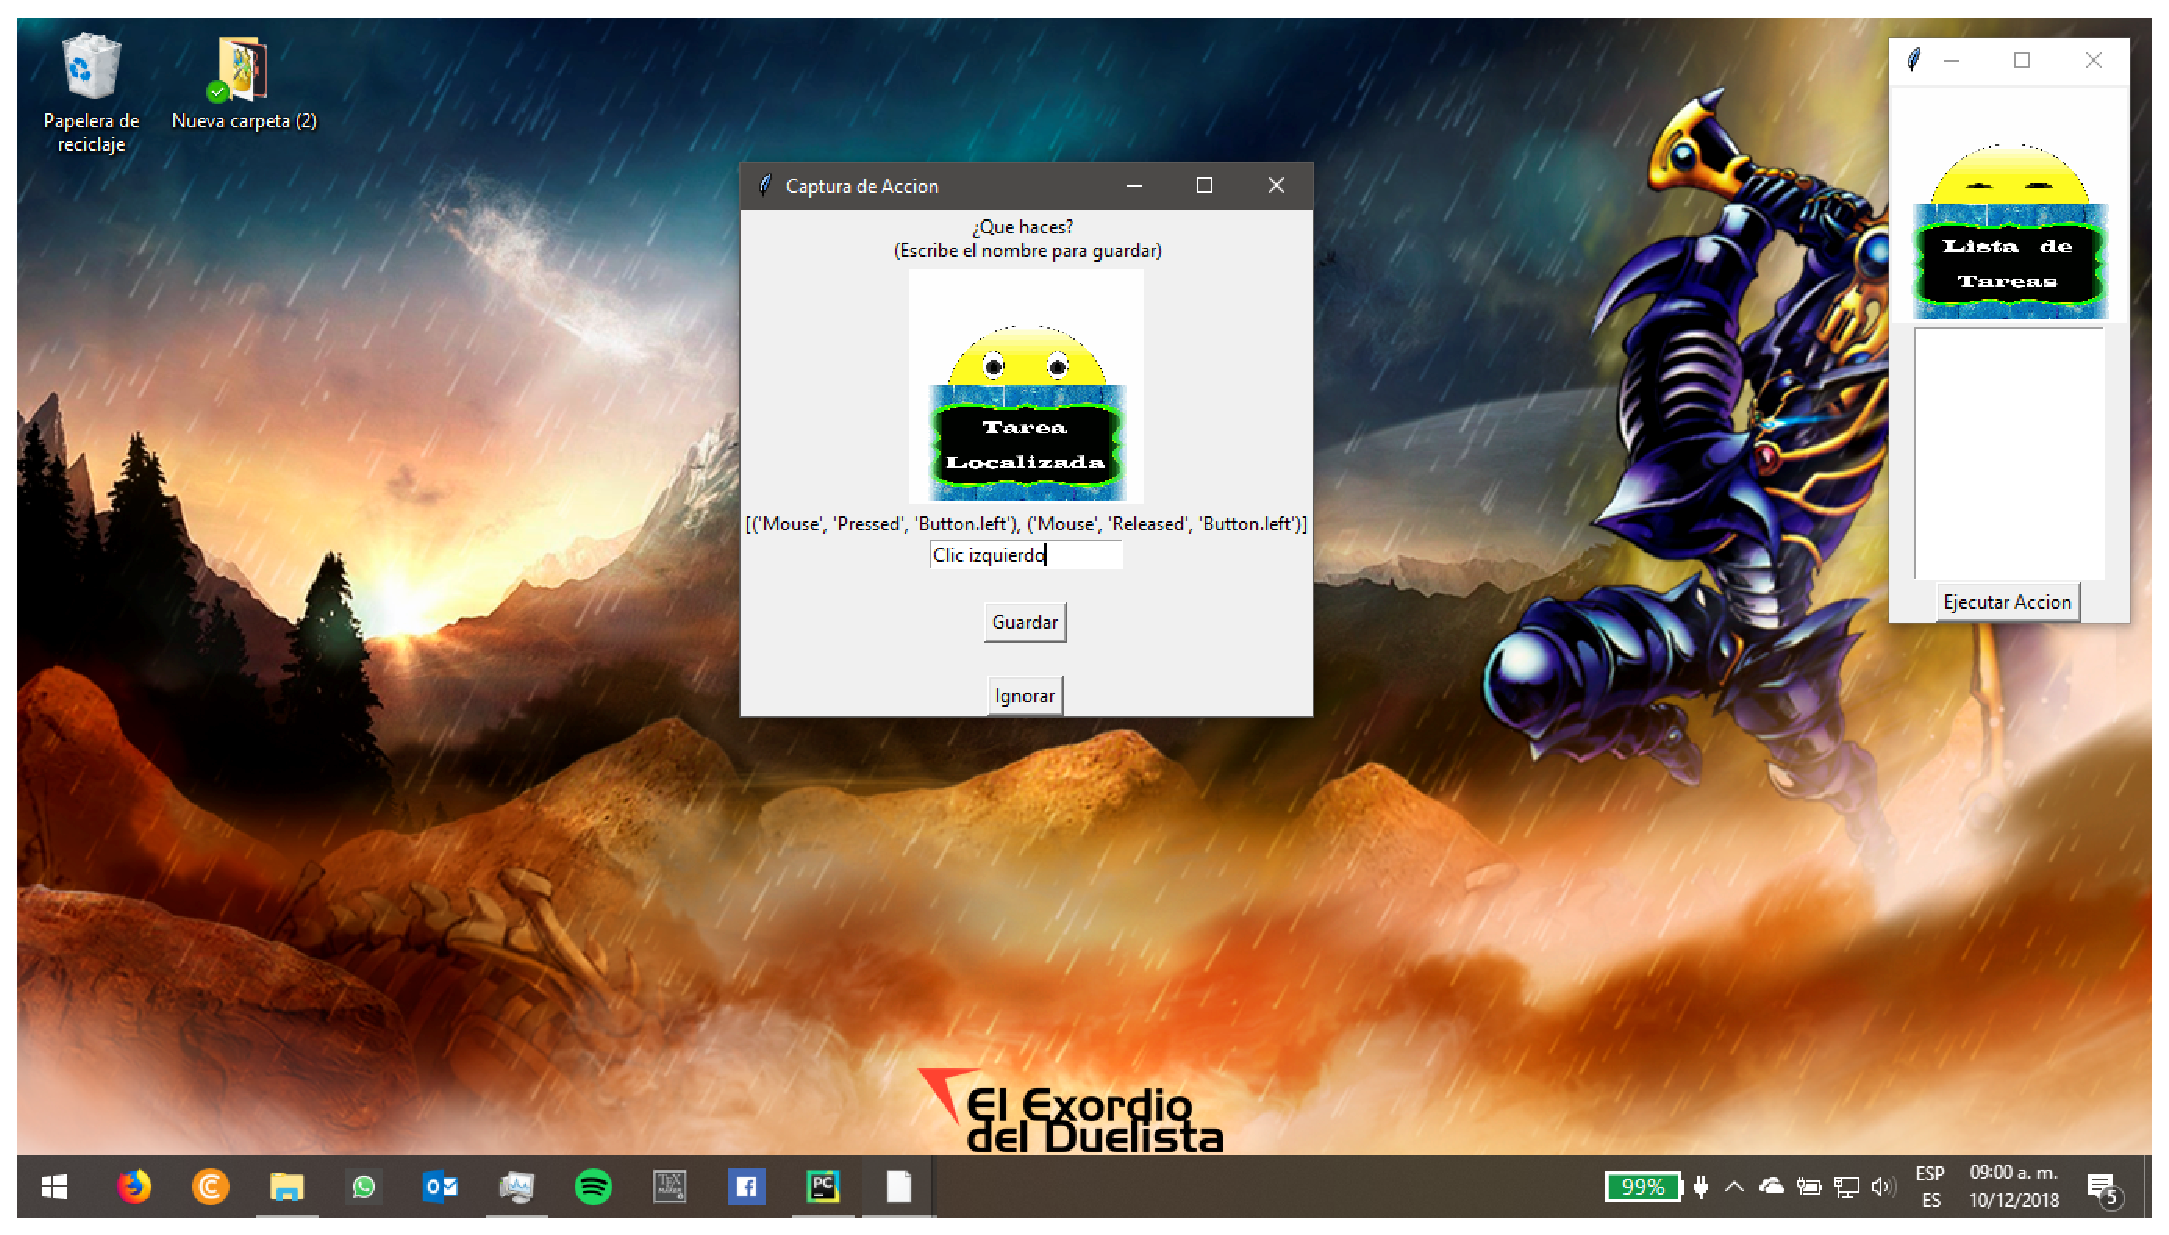
\includegraphics[width=1.0\columnwidth]{Imagenes/5.eps}
\end{figure}
\end{frame}

\begin{frame}
\frametitle{Demostraci\'on}
\begin{figure}[H]
\centering
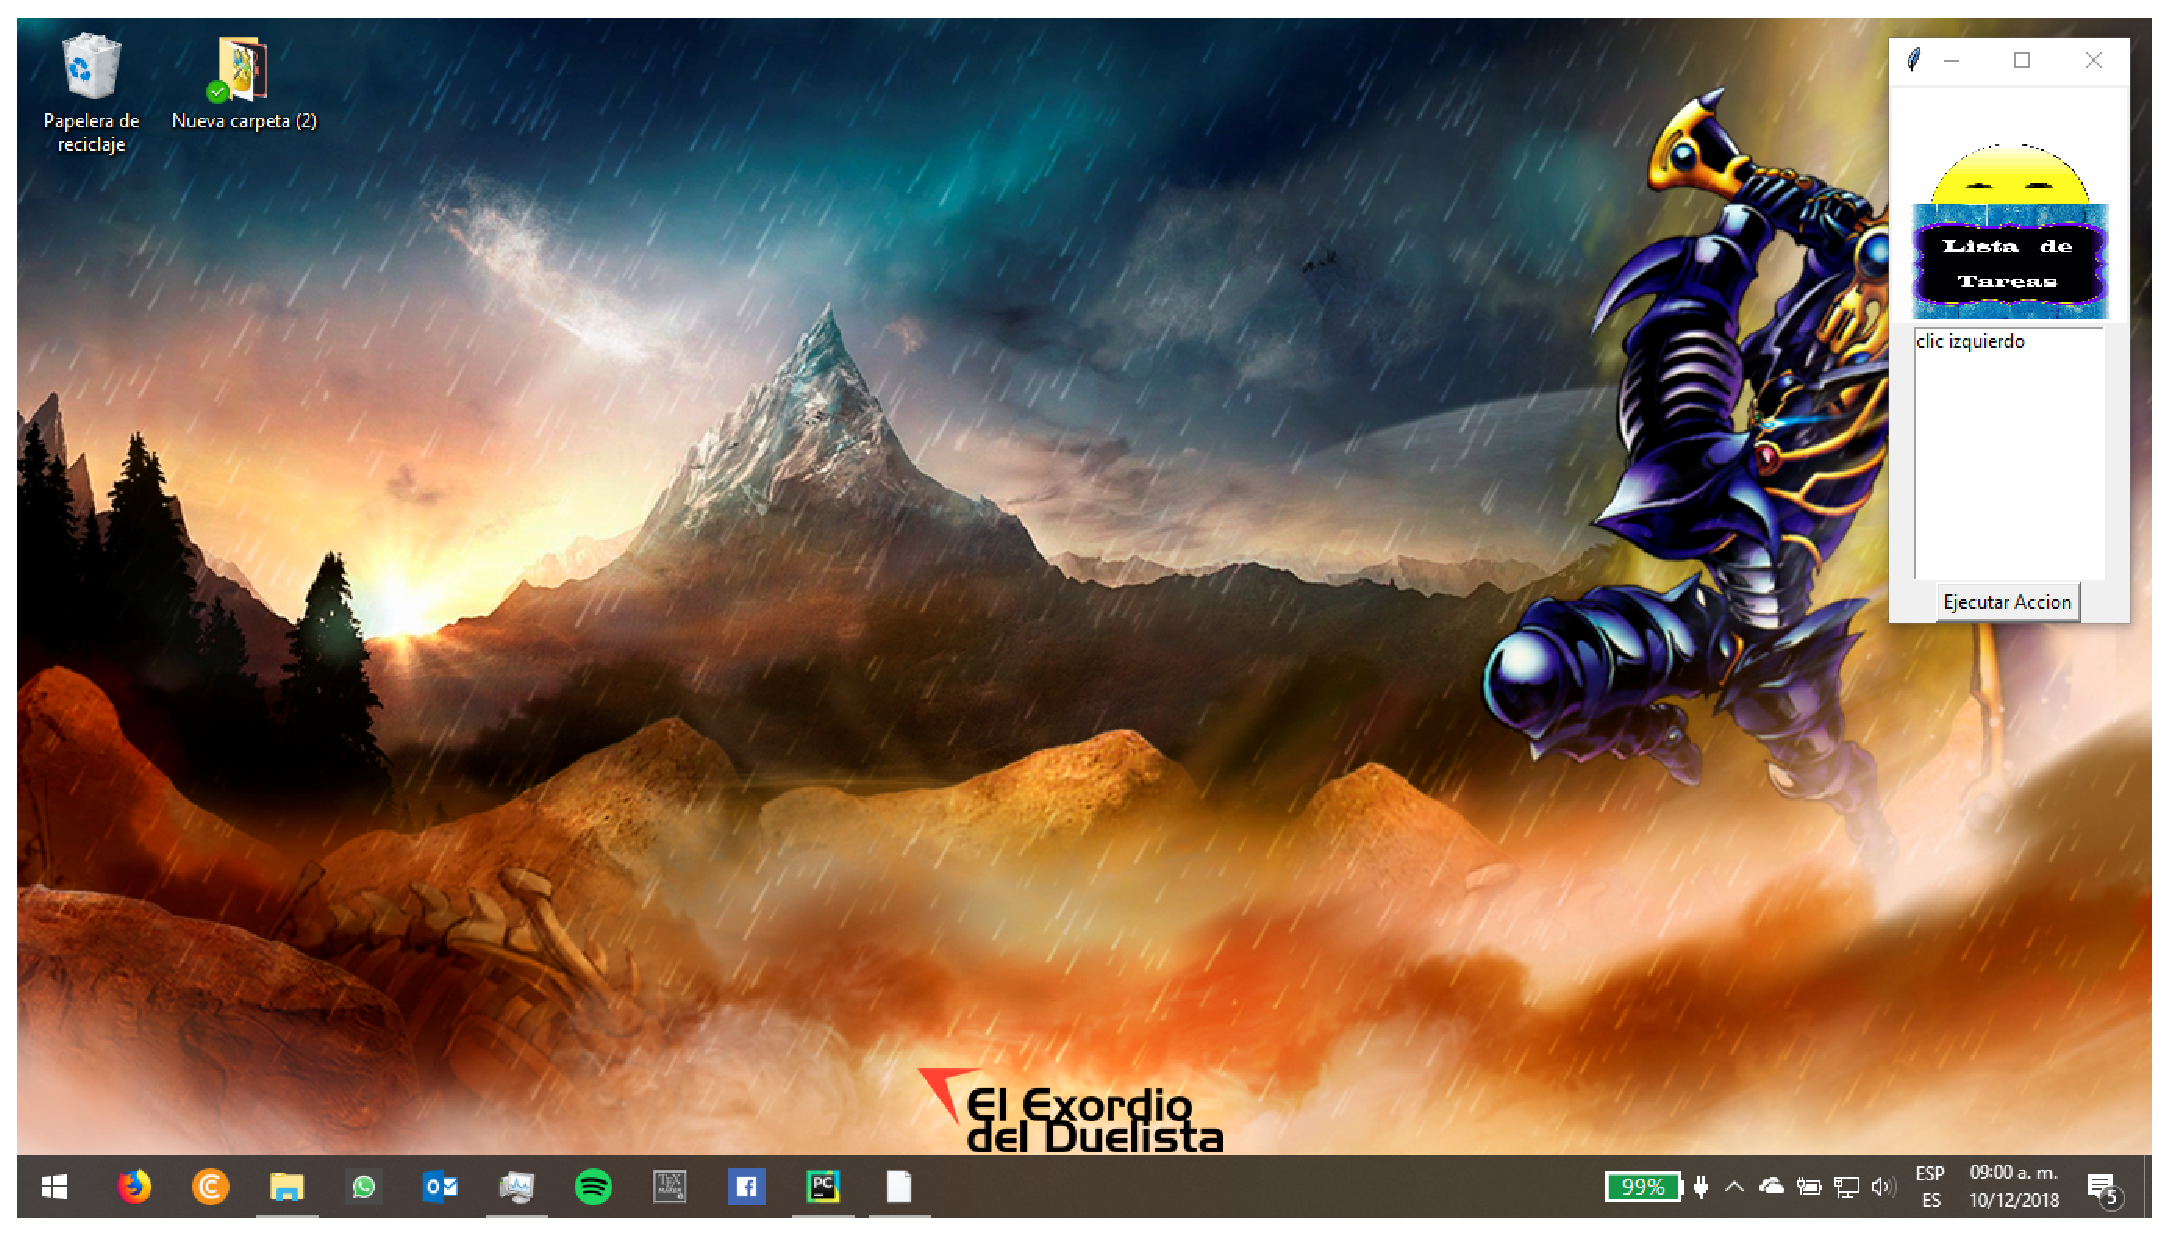
\includegraphics[width=1.0\columnwidth]{Imagenes/6.eps}
\end{figure}
\end{frame}

\begin{frame}
\frametitle{Demostraci\'on}
\begin{figure}[H]
\centering
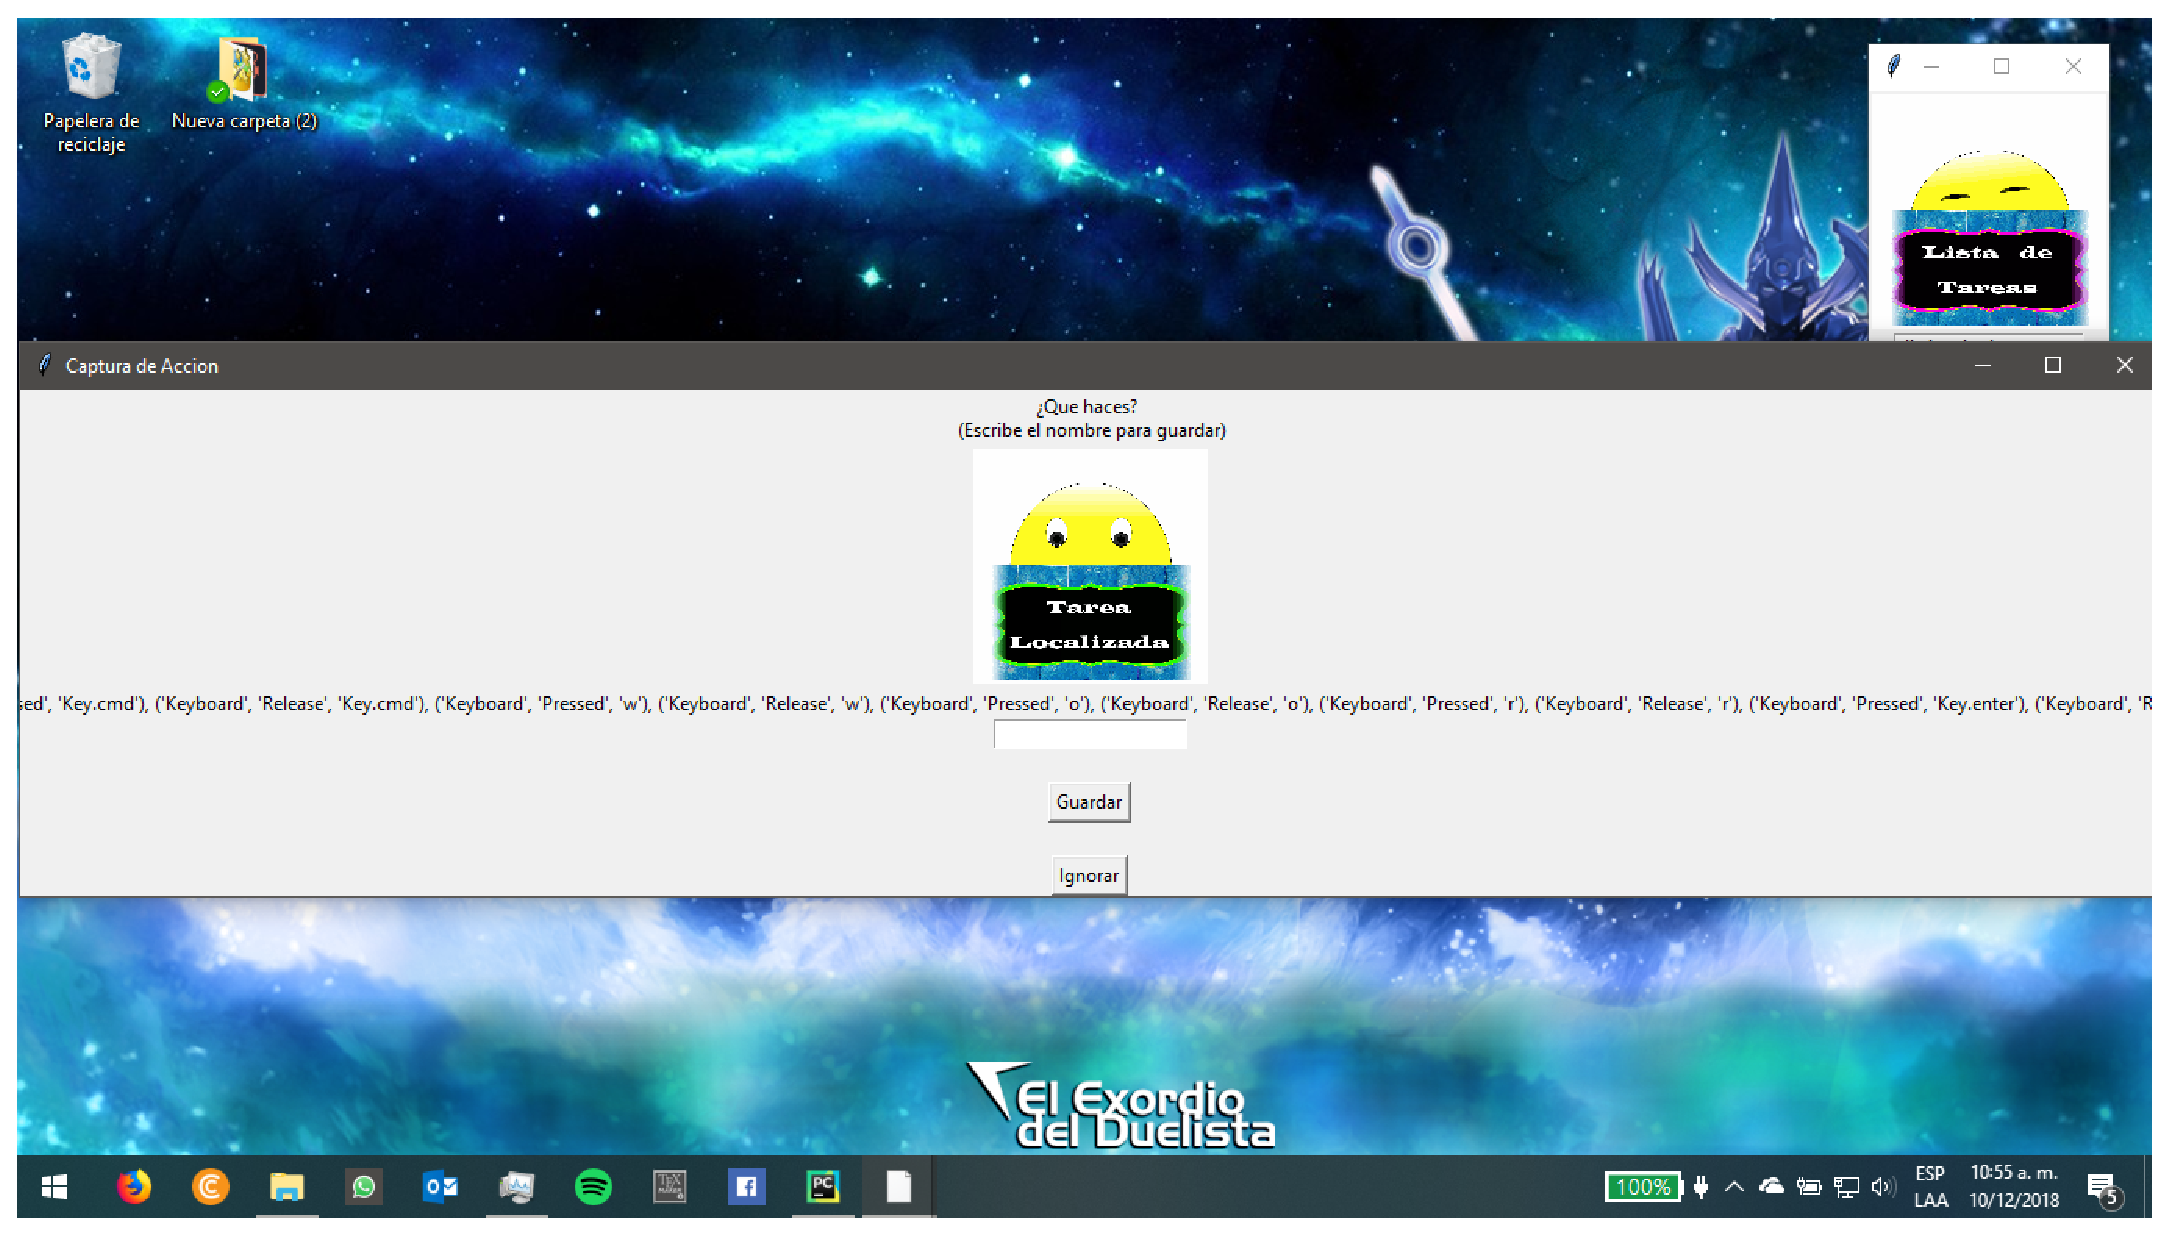
\includegraphics[width=1.0\columnwidth]{Imagenes/7.eps}
\end{figure}
\end{frame}

\begin{frame}
\frametitle{Demostraci\'on}
\begin{figure}[H]
\centering
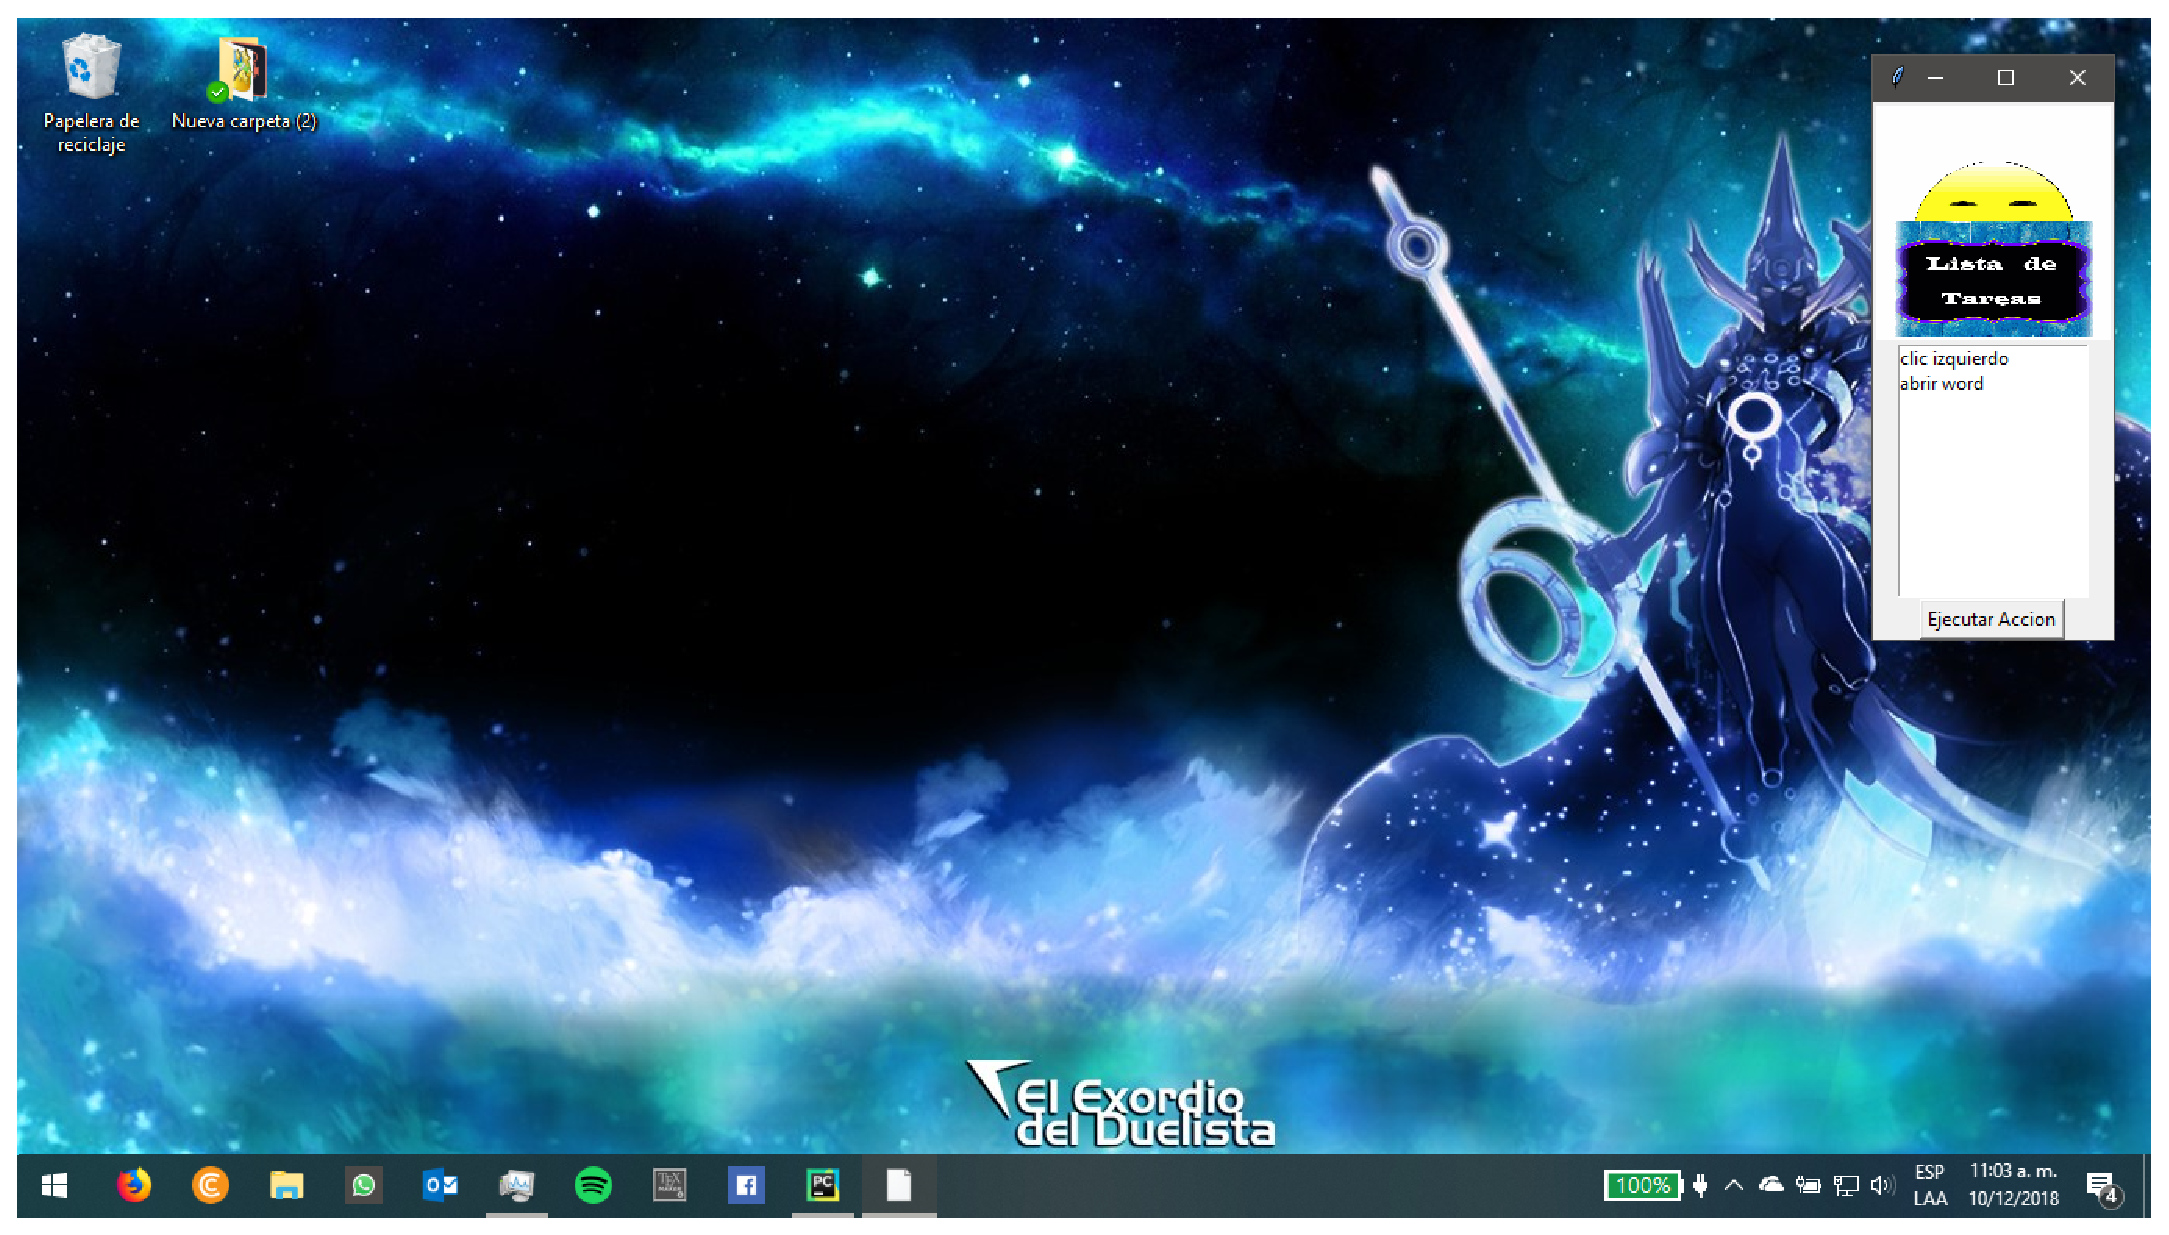
\includegraphics[width=1.0\columnwidth]{Imagenes/8.eps}
\end{figure}
\end{frame}


\section{Experimentos y resultados}

\subsection{Introducci\'on}
\begin{frame}
\frametitle{Experimentos}

\begin{table}[]
\centering
\scalebox{0.8}{
\begin{tabular}{cccc}
\hline
No. de Sujeto	
&   Tiempo de Uso (Hr:Min)		
&	N\'umero de Nodos	
&   Repeticiones 	\\   
\hline

1				
&	166:23 						
&	1,494,792			
&	46,036				\\
		
2
&	490:24
&	1,333,016
&	116,001				\\
		
3
&	1060:48
&	1,448,016
&	378,541				\\
		
4
&	148:23
&	972,828
&	56,606				\\ 
\hline

\end{tabular}
}
\caption{Informaci\'on de los datos recabados.}
\label{infodata}
\end{table}

\begin{block}{Condiciones:}
\centering
\begin{itemize}
\item {70 incidencias en el nodo}
\item {5 repeticiones de la secuencia}
\item {No \textbf{empezar} con \emph{Release}}
\item {No \textbf{terminar} con \emph{Pressed}}
\end{itemize}
\end{block}

\end{frame}


\begin{frame}
\frametitle{Resultados}
\begin{table}[]
\centering
\scalebox{0.75}{
\begin{tabular}{cccc}
\hline
\textbf{No. de }	
&	\textbf{Secuencias }	
&   \textbf{Secuencias }	
&	\textbf{Porcentaje de }	\\

\textbf{Sujeto}
&	\textbf{Aceptables}
&	\textbf{Totales}
&	\textbf{Precisi\'on}
	\\ \hline

1				
&	189						
&	525						
&	36.00 \%		\\

2				
&	165						
&	487						
&	33.88 \%		\\

3
&	151
&	467
&	32.33 \%		\\

4
&	56
&	180
&	31.11 \%		\\
\hline
\end{tabular}
}
\caption{Tabla de resultados con secuencias de una longitud m\'inima de 
 1 acci\'on.}
\label{tableRes1}
\end{table}


\begin{table}[]
\centering
\scalebox{0.75}{
\begin{tabular}{cccc}
\hline
\textbf{No. de }	
&	\textbf{Secuencias }	
&   \textbf{Secuencias }	
&	\textbf{Porcentaje de }	\\

\textbf{Sujeto}
&	\textbf{Aceptables}
&	\textbf{Totales}
&	\textbf{Precisi\'on}
	\\ \hline

1
&	179
&	410
&	43.65 \%		\\
	
2
&	170
&	377
&	45.09 \%		\\

3
&	154
&	346
&	44.50 \%		\\

4
&	52
&	119
&	43.69 \%		\\
\hline
\end{tabular}
}
\caption{Tabla de resultados con secuencias de una longitud m\'inima de 
 2 acciones.}
\label{tableRes2}
\end{table}



\end{frame}


\begin{frame}
\frametitle{Resultados}

\begin{columns}[T]
		\begin{column}{.33\textwidth}
			\begin{block}{\small{Es la palabra ``el''}}
				\centering
				Keyboard,Pressed,e	\\
				Keyboard,Release,e	\\
				Keyboard,Pressed,l	\\
				Keyboard,Release,l	\\
			\end{block}
		\end{column}

		\begin{column}{.33\textwidth}
			\begin{block}{\small{ La tarea es utilizada en el software
			 Blender para girar el objeto en el eje Y}}
				\centering
				Keyboard,Pressed,G\\
				Keyboard,Release,G\\
				Keyboard,Pressed,Y\\
				Keyboard,Release,Y\\
			\end{block}
		\end{column}
		
		\begin{column}{.33\textwidth}
			\begin{block}{\small{En Windows es utilizada esta combinaci\'on
			 de teclas para cambiar entre las ventanas abiertas.}}	
				\centering
				Keyboard,Pressed,alt\_l	\\
				Keyboard,Pressed,tab	\\
				Keyboard,Release,tab	\\
				Keyboard,Release,alt\_l	\\
			\end{block}
		\end{column}
		
	\end{columns}
\end{frame}


\subsection{Discusi\'on}
\begin{frame}
\frametitle{Discusi\'on}

\begin{table}[h]
\centering
\scalebox{0.9}{
\begin{tabular}{m{5cm}|m{5cm}}
\hline
\textbf{Creador de macros}
&
\textbf{Software desarrollado} \\
\hline
Hay que indicar manualmente cuando empieza y termina la acci\'on deseada	
 &	
Se monitorea cada acci\'on realizada por el usuario.\\
\hline

El usuario graba manualmente la tarea que desea automatizar	
 &
Se muestra al usuario las acciones que realiza con mayor frecuencia para que
  \'el decida cual guardar\\
\hline

El usuario requiere conocimiento del software para crear tareas complejas 	
 &
El usuario no requiere editar las tareas\\
\hline
\end{tabular}
}
\caption{An\'alisis comparativo del software con un generador de macros.}
\label{vsmacros}
\end{table}

\end{frame}


\begin{frame}
\frametitle{Discusi\'on}

\begin{table}[h]
\centering
\scalebox{0.9}{
\begin{tabular}{m{5cm}|m{5cm}}
\hline
\textbf{Robotic Process Automation}
&
\textbf{Software desarrollado} \\

\hline
Hay que indicar manualmente cuando empieza y termina la acci\'on deseada.
&
Se monitorea cada acci\'on realizada por el usuario.\\

\hline
Por medio de t\'ecnicas de reconocimiento de im\'agenes y monitoreo a los
 dispositivos de E/S, se determina la acci\'on realizada y el momento de 
 ejecuci\'on. 
&
Por medio del an\'alisis en tiempo ejecuci\'on de un grafo dirigido se 
 obtienen las tareas realizadas.\\

\hline
Se automatiza un proceso en espec\'ifico.
&
Se automatiza la tarea que m\'as realice el usuario.\\

\hline
\end{tabular}
}
\caption{An\'alisis comparativo de la propuesta con Robotic Process
 Automation.}
\label{vsrpa}
\end{table}

\end{frame}
\section{Conclusiones}

\begin{frame}
\frametitle{Conclusiones}
\begin{itemize}
\item {
Se implement\'o un sistema de captura para el teclado y rat\'on, con el cual
 se obtuvo la informaci\'on de 4 sujetos en el plazo de 3 meses para 
 realizar las pruebas mencionadas.
}
\item {
Se dise\~n\'o un algoritmo de aprendizaje no supervisado que no tiene un
 tiempo de finalizaci\'on determinado, el aprendizaje es continuo, durante la 
 ejecuci\'on obtiene secuencias de acciones realizadas por un usuario, sin 
 datos de ejemplo. Los resultados experimentales demuestran que el software 
 desarrollado es capaz de proporcionar tareas \'utiles para la 
 automatizaci\'on de las mismas, independientemente del software que este 
 usando la persona, de forma que en una lista pseudo--infinita de datos 
 ordenados por momento de aparici\'on, es posible encontrar secuencias de 
 informaci\'on coherente para un usuario.
}
\end{itemize}
\end{frame}

\begin{frame}
\frametitle{Conclusiones}
\begin{itemize}
\item{
Se plante\'o la b\'usqueda de sistemas similares en la cual no se logr\'o 
 el \'exito esperado, dejando como sistemas similares a los creadores de
 macros y RPA, por lo que no se encontraron los elementos necesarios 
 para realizar un an\'alisis comparativo de resultados.
}
\item {
En la hip\'otesis propuesta se menciona que los humanos son seres de 
 costumbres por lo que el software propuesto debe de reconocer esos h\'abitos, 
 pero considerando que en las secuencias obtenidas solo hay registro de teclas
 y botones del teclado y rat\'on respectivamente, lo cual implica que los
 movimientos con el rat\'on no son tan mec\'anicos como se esperaba.
}
\end{itemize}
\end{frame}


\subsection{Trabajos futuros}
\begin{frame}
\frametitle{Trabajos futuros}

\begin{itemize}
	\item Mejora a la interfaz usuario--maquina
	\item Mejora al reconocimiento de tareas
	\item Mejora a la ejecuci\'on de tareas
	\item Exploraci\'on en otras areas
\end{itemize}

\end{frame}

\subsection{Productos de la investigaci\'{o}n}
\begin{frame}
\frametitle{Productos de la investigaci\'{o}n}

\begin{itemize}
\scriptsize
\item {Gonz\'alez Tello; R., Chan Alejandre; E. A., Serrano Talamantes; J. 
 F.,\& Carbajal, Olgu\'in; M. (2016, May). COMPUTACI\'ON INTELIGENTE: UN 
 ESTUDIO COMPARATIVO DE METAHEUR\'ISTICAS. Bolet\'in UPIITA No. 66. Retrieved 
 from http://www.boletin.upiita.ipn.mx/index.php/ciencia/762-cyt-numero-66/1519-computacion-inteligente-un-estudio-comparativo-de-metaheuristicas}

\item {Chan Alejandre, E. A., Rivera Z\'arate, I., Olgu\'in Carbajal, M., \&
 Gonz\'alez Tello, R. (2017, Sep). Electronic impact system for a football 
 player\textsc{\char13}s helmet. In 17th International Congress on Computer 
 Science (p. 8). M\'exico: Centro de Investigac\'on en Computaci\'on.}

\item {Chan Alejandre, E. A., Rivera Z\'arate, I., Olgu\'in Carbajal, M., \& 
 Gonz\'alez Tello, R. (2017, Sep). SISTEMA MEDIDOR ELECTR\'ONICO DE IMPACTOS 
 PARA CASCO DE FUTBOL AMERICANO POR MEDIO DE ACELEROMETROS. In XVIII 
 Simposium Internacional : ``Aportaciones de la universidades a la docencia, 
 la investigaci\'on, la tecnolog\'ia y el desarrollo'' (p. 5). M\'exico: 
 Escuela Superior de Ingenier\'ia Qu\'imica e Industrias Extractivas.}
 
\end{itemize}


\end{frame}


\section{Referencias}
\begin{frame}
\Huge
\centering
Referencias
\end{frame}
\bibliographystyle{plain}
\tiny
\bibliography{Bibliografia}




\begin{frame}
\centering
\begin{Huge}
Gracias
\end{Huge}
\end{frame}

\end{document}
